\documentclass[a4paper,polish]{article}

%\newcommand{\DoNotLoadEpstopdf}{}

\usepackage[T1]{fontenc}
\usepackage{polski}
\usepackage[polish]{babel}
\usepackage[margin=3cm]{geometry}
\usepackage{graphicx}
\usepackage[utf8]{inputenc}
\usepackage{hyphenat}
\usepackage{amsmath}
\usepackage{amsfonts}
\usepackage{titlesec}
\usepackage{csquotes}
\usepackage{indentfirst}
\usepackage{datetime}
\usepackage{mathtools}
\usepackage{xparse,eqparbox,amsmath}
\usepackage{color}
\usepackage{setspace}
\usepackage[nottoc,numbib]{tocbibind}

\usepackage{cite}  %added by P.J.

\setstretch{1.3}

\selectlanguage{polish}

\usepackage{subfig}


%-------Definition of \signature--
 \def\signature#1#2#3{{\hskip#1in{\hbox to #2in%
{\leaders\hbox to .00625in{\hfil.\hfil}\hfill}}%
 \par\hskip#1in#3\vskip1cm}}
%------------------------------
% https://tex.stackexchange.com/a/34412/5764
\makeatletter
\NewDocumentCommand{\eqmathbox}{o O{c} m}{%
	\IfValueTF{#1}
	{\def\eqmathbox@##1##2{\eqmakebox[#1][#2]{$##1##2$}}}
	{\def\eqmathbox@##1##2{\eqmakebox{$##1##2$}}}
	\mathpalette\eqmathbox@{#3}
}

% copied from article.cls, added \boldmath
\renewcommand\subsubsection{\@startsection{subsubsection}{3}{\z@}%
	{-3.25ex\@plus -1ex \@minus -.2ex}%
	{1.5ex \@plus .2ex}%
	{\normalfont\normalsize\bfseries\boldmath}}

\makeatother

\newcommand{\ts}{\quad}

%-------Big chapter letters--
\titleformat{\chapter}[display]
  {\huge\headingfont}{\chaptertitlename\ \thechapter}{20pt}{\Huge}
%------------------------------

\frenchspacing

\numberwithin{equation}{section}

\begin{document}

\begin{titlepage}
	\renewcommand{\baselinestretch}{1} 
	\centering
	\begin{figure}[t]
	\centering
	
\includegraphics[width=0.25\textwidth]{logo_uz}
	\end{figure}
	\vspace{1cm}
	{\scshape\huge Uniwersytet Zielonogórski \par}
	{\scshape\LARGE Wydział Fizyki i Astronomii \par}
	{\scshape\Large Instytut Fizyki \par}
	\vspace{1.5cm}
	{\Large\bfseries Wyznaczanie mas dla stanów podstawowych ciężkich jąder atomowych w ramach modelu makroskopowo-mikroskopowego z wykorzystaniem parametryzacji modif{}ied Funny-Hills. \par}
	\vspace{1cm}
	{\Large\textbf{Dawid Haniewicz} \par}
	\vspace{2cm}
	Praca inżynierska napisana \par
	pod przewodnictwem: dra~Piotra \textsc{Jachimowicza} \par
	\vspace{1.5cm}
	{Kierunek: \textsc{\textbf{Fizyka Techniczna}} \par}
	{Specjalność: \textsc{\textbf{Fizyka Medyczna}} \par}
	\vspace{1.5cm}
	Akceptacja promotora: \par
	\vspace{0.5cm}
	\signature{0}{1.8}
	\vfill
% Bottom of the page
	{\large Zielona Góra, \the\year \par}
	\thispagestyle{empty}
\end{titlepage}

\setcounter{page}{2}

\clearpage
\tableofcontents
\clearpage

%\chapter{po angielsku}
%To describe the ground state shapes and not very elon-
%gated fission barriers particularly frequently expansion in
%spherical harmonics has been used. This allows to in-
%clude a mixing of various multipolarities when considering
%exotic shapes. On the other hand the more elongated
%shapes the more independent parameters should be taken
%into account.



%{ \LARGE

%Tematem pracy jest ... 
%\\

%The aim of the bachelor's thesis is ... 
%}

\section{Streszczenie pracy inżynierskiej - Abstract of bachelor thesis}

Tematem niniejszej pracy jest wyznaczanie mas dla stanów podstawowych ciężkich jąder atomowych w ramach modelu makroskopowo-mikroskopowego z wykorzystaniem parametryzacji modified Funny-Hills. Celem pracy jest sprawdzenie działania tej parametryzacji w opisie energii/mas dla stanów podstawowych wybranych ciężkich jąder atomowych. Praca składa się z pięciu rozdziałów. Pierwszy z nich to wprowadzenie, w którym dokładniej opisuję cel swojej pracy. Drugi rozdział to wstęp teoretyczny, w którym w oparciu o literaturę opisuję część makroskopową oraz mikroskopową energii nuklidu. Jest on szczególnie istotny ponieważ w oparciu o te założenia budowane są modele. Trzeci rozdział jest rozdziałem, który opisuje obydwie stosowane przeze mnie parametryzacje – beta oraz modified Funny-Hills, ich zastosowanie oraz sposób przeliczania jednej w drugą. W rozdziale czwartym ukazane są przykłady konwersji kształtów parametryzacji  modified Funny-Hills do rozwinięcia beta. Rozdział ten zawiera również szczegółowy opis wyników obliczeń mas dla wybranych ciężkich jąder atomowych. W ostatnim rozdziale podsumowuję swoją pracę oraz wyciągam wnioski na podstawie uzyskanych wyników obliczeń. Celem przeprowadzonych obliczeń było sprawdzenie poprawności działania parametryzacji modified Funny-Hills w oparciu o częściowo istniejące dane eksperymentalne. Obliczenia przeprowadzono dla dwóch znanych nuklidów oraz na jednym abstrakcyjnym.
\\

The theme of this presentation is determination of masses for the basic states of heavy atomic nuclei within the macroscopic-microscopic model using modified Funny-Hills parameterization. The purpose of the bachelor's thesis is to check the operation of this parameterization in the description of energy/mass for basic states of selected heavy atomic nuclei. The work consists of five chapters. The first one is an introduction, in which I describe in more details the purpose of my work. The second section is a theoretical introduction, in which I describe the macroscopic and microscopic part of nuclide energy on the basis of literature. It is particularly important because models are built on these principles. The third section is a chapter that describes both my beta and modified Funny-Hills parameters, their use, and how to convert them from one to another. The fourth section shows examples of converting modified Funny-Hills parametrization shapes to beta expansion. This chapter also contains a detailed description of the results of mass calculations for selected heavy atomic nuclei. In the last chapter I summarize my work and draw conclusions based on the results of the calculations. The purpose of the calculations was to verify the correct operation of the modified Funny-Hills parameterization based on partially existing experimental data. Calculations were made for two known nuclides and one abstract.

\clearpage
\section{Wprowadzenie}

W chwili obecnej znanych jest około 3000 jąder atomowych z czego większość z nich to nuklidy zdeformowane, tj. charakteryzujące się w stanach podstawowych kształtami odbiegającymi od sfery. Przykładem tego mogą być jądra z grupy ziem rzadkich lub rozległy obszar aktynowców, dla których już od wielu lat obserwuje się widma stanów rotacyjnych  jak i dokonuje pomiarów elektrycznych momentów multipolowych - istnienie elektrycznego momentu kwadrupolowego jądra atomowego zostało eksperymentalnie wykryte już w 1935 r. \cite{1935}.

Umiejętność opisu jądrowej deformacji ma fundamentalne znaczenie dla odtwarzania i przewidywania wielu własności jądrowych, zarówno tych strukturalnych jak i spektroskopowych. Opisu tego dokonuje się poprzez wybór odpowiedniej parametryzacji, tj. poprzez rozwinięcie powierzchni jądra w skończony szereg liczb, tak aby możliwym było wykorzystanie ich jako zmiennych w obliczeniach numerycznych. Historycznie pierwsza taka parametryzacja, polegająca na uzależnieniu energii wiązania od kształtu nuklidu, wprowadzona została przez N. Bora i J. Wheelera w 1939 r. \cite{1939} i była następstwem odkrycia zjawiska rozszczepienia uranu. Od tego czasu wprowadzono wiele różnych parametryzacji, np. \cite{parametryzacje}, dostosowanych do konkretnych typów zjawisk lub obszarów nuklidów. Wybór odpowiedniej z nich powinien być uzasadniany przede wszystkim typem kształtów mogących mieć znaczenie w badanym obszarze nuklidów, lecz i także możliwie dużą prostotą obliczeń.

W przypadku jąder najcięższych, dla których duża liczba protonów i związane z tym odpychanie kulombowskie zasadniczo uniemożliwia zbytnie odejście od kształtów sferycznych, stosunkowo dobrą parametryzację stanowi rozwinięcie powierzchni jądra w szereg funkcji kulistych - tj. tzw. parametryzacja $\beta$. Ze względów numerycznych taki szereg powinien być oczywiście skończony. W praktyce jest to równoznaczne z wybraniem z niego tylko pewnych typów kształtów, przy założeniu, że są one ,,najważniejsze'' oraz na odrzuceniu pozostałych, uznawanych za mniej ważne. Mimo oczywistych wad opisana parametryzacja bardzo dobrze sprawdza się np. w przypadku wyznaczania mas/energii stanów podstawowych, natomiast w przypadku znacznego odejścia od sfery, np. próbach opisu jąder charakteryzujących się długimi barierami rozszczepieniowymi, parametryzacja ta może wymagać uwzględnienia wielu typów kształtów (tj. stopni swobody), utrudniając tym samym obliczenia \cite{Jach1}, lub czyniąc je nawet niemożliwymi do wykonania w sposób rzetelny. Ratunkiem w tej sytuacji może być użycie innej parametryzacji, np. tzw. parametryzacji modified Funny-Hills, wprowadzonej przez K. Pomorskiego i J. Bartela \cite{MFH}, stanowiącej rozwinięcie parametryzacji Funny-Hills \cite{OLDMFH} i wykorzystującej tylko cztery odpowiednio dobrane parametry: $c, h, \alpha, \eta$, których znaczenie i sens fizyczny omówione zostaną w dalszej części pracy. Parametryzacja ta nadaje się zarówno do opisu kształtów charakteryzujących się znacznym wydłużeniem, lecz i także, zgodnie z twierdzeniem autorów \cite{MFH}, do opisu kształtów bliskich sfery, tj. np. wyznaczania energii/mas dla stanów podstawowych.

\clearpage
\subsection{Cel pracy oraz sposób jego realizacji}

Celem niniejszej pracy jest więc sprawdzenie działania parametryzacji modified Funny-Hills w opisie energii/mas dla stanów podstawowych wybranych nuklidów. Warto w tym miejscu wspomnieć, że nie każda parametryzacja dobrze sprawdzająca się w opisie kształtów silnie wydłużonych, tj. bliskich rozszczepieniu, nadaje się także do opisu niewielkich wydłużeń. Przykładem tego może być tzw. parametryzacja three quadratic surfaces, wprowadzona przez J. R. Nixa \cite{NIX}, która w przypadku niewielkich deformacji prowadzi do znacznych błędów i jest najczęściej zastępowana parametryzacją $\beta$, np. \cite{Moll2009}.

Samo wyznaczanie energii/mass jądrowych w niniejszej pracy opierać się będzie na tzw. modelu makroskopowo-mikroskopowym, który szczegółowo opisany został w następnym rozdziale. Model ten z powodzeniem wykorzystywany jest już od wielu lat do opisu różnego rodzaju własności jądrowych, np. \cite{JACHQ,JACHBF,Muntian}, a odpowiadający mu kod numeryczny, który będę tu wykorzystywał, opiera się na parametryzacji $\beta$. Ponieważ przepisanie wspomnianego kodu na inną parametryzację znacznie przekracza zakres pracy inżynierskiej, sprawdzenie działania parametryzacji modified Funny-Hills opierać się tu będzie na umiejętnym i bardzo precyzyjnym przeliczeniu wygenerowanego w ramach jej kształtu (definiowanego przez parametry $c, h, \alpha, \eta$),  na parametryzację $\beta$, tak aby możliwe było użycie wspomnianego kodu numerycznego (tj. modelu makroskopowo-mikroskopowego), bez potrzeby wprowadzania do niego większych modyfikacji. Szczegółowy opis sposobu przeliczania parametryzacji modified Funny-Hills na parametryzację $\beta$ znajduje się na końcu rozdziału 3 niniejszej pracy.

\section{Model mikroskopowo-makroskopowy}

W niniejszej pracy energia potencjalna (masa) jądra atomowego obliczana jest w ramach podejścia makroskopowo-mikroskopowego. Zgodnie z nim energia (masa) jądra składa się z dwóch części, makroskopowej $E\textsubscript{macr}$, zmieniającej się gładko przy przejściu od jądra do jądra, oraz silnie fluktuującej poprawki do części makroskopowej: $E\textsubscript{micr}$, ujmującej efekty powłokowe wynikające z kwantowej natury jądra atomowego: 

\begin{equation}
E\textsubscript{mm}(Z,N,\beta_{\lambda \mu}) = E\textsubscript{macr}(Z,N,\beta_{\lambda \mu}) + E\textsubscript{micr}(Z,N,\beta_{\lambda \mu}).
\end{equation}
Każda ze wspomnianych części zależna jest od liczby atomowej $Z$, liczby neutronów $N$ oraz kształtu (deformacji) nuklidu $\beta_{\lambda \mu}$.

\subsection{Część makroskopowa energii}
Gładka (makroskopowa) część energii jądra wyznaczana jest w ramach modelu kroplowego Yukawa-plus exponential \cite{Krappe} mającego w przypadku jąder parzysto-parzystych następującą formę:

\begin{equation} \label{Eq:Yukawa_model}
\begin{gathered}
M_{makr}(Z,N,\beta^0_{\lambda})=M_{H}Z+M{n}N-a_{V}(1-\kappa_{V}I^2)A+a_{s}(1-\kappa_{s}I^2)A^{2/3}B_{1}(\beta^{0}_{\lambda}) \\
+a_{0}A^{0}+c_{1}Z^{2}A^{-1/3}B_{3}(\beta^{0}_{\lambda})-c_{4}Z^{4/3}A^{-1/3} \\
+f(k_{F}r_{r})Z^{2}A^{-1}-c_{a}(N-Z)-a_{el}Z^{2.39}
\end{gathered}
\end{equation}
gdzie $M_{H}$ to masa atomu wodoru, $M_{n}$ - masa neutronu, parametr $I=(N-Z)/A$ wyznacza względny nadmiar neutronów nad protonami, natomiast $A=Z+N$ to liczba masowa. Funkcje $B_{1}(\beta_{\lambda})$ i $B_{3}(\beta_{\lambda})$ opisują odpowiednio zależność: członu powierzchniowego i członu kulombowskiego od deformacji jądra:
\begin{gather}
B_{1}=\frac{A^{-2/3}}{8\pi^{2}r^{2}_{0}a^{4}}\iint_V\left(2-\frac{r_{12}}{a}\right)\frac{e^{-r_{12}/a}}{r_{12}/a}d^{3}r_{1}d^{3}r_{2} \\
B_{3}=\frac{15}{32\pi^{2}}\frac{A^{-5/3}}{r^{5}_{0}}\iint_V\frac{1}{r_{12}}\left[1-\left(1+\frac{1}{2}\frac{r_{12}}{a_{den}}\right)e^{-r_{12}/a_{den}}\right]d^{3}r_{1}d^{3}r_{2},
\end{gather}
gdzie $r_{12}=\left|\vec{r_{1}}-\vec{r_{2}}\right|$ jest odległością pomiędzy oddziałującymi 
elementami objętości wyznaczanymi przez wektory $\vec{r_{1}}$ i $\vec{r_{2}}$. Funkcje te dobrane 
są w taki sposób, że dla kształtu sferycznego i przy założeniu ostrego brzegu powierzchni jądra, tj. $a=0$ oraz $a_{den}=0$, są one równe 1. Współczynniki $c_{1}$ i $c_{4}$ pojawiające się we wzorze (\ref{Eq:Yukawa_model}) zdefiniowane są w następujący sposób:
\begin{equation}
c_{1}=\frac{3}{5}\frac{e^{2}}{r_{0}}, \qquad c_{4}=\frac{5}{4}\left(\frac{3}{2\pi}\right)^{2/3}c_{1},
\end{equation}
gdzie $e$ to elementarny ładunek elektryczny a $r_{0}$ opisuje promień jądra. Funkcja $f(k_{F}r_{p})$ będąca tzw. czynnikiem postaci zdefiniowana jest jako:
\begin{equation}
f(k_{F}r_{p})--\frac{1}{8}\frac{e^{2}r^{2}_{p}}{r^{3}_{0}}\left[\frac{145}{48}-\frac{327}{2880}(k_{F}r_{p})^{2}+\frac{1527}{1209600}(k_{F}r_{p})^{4}\right],
\end{equation}
gdzie $k_{F}$ to długość wektora falowego Fermiego:
\begin{equation}
k_{F}=\left(\frac{9\pi Z}{4A}\right)^{1/3}r^{-1}_{0},
\end{equation}
natomiast $r_{p}$ jest średnią kwadratową promienia protonu. 

Poszczególne parametry używane w niniejszym modelu przyjęto zgodnie z \cite{Moll1,Moll2} i mają one następujące wartości:

\begin{gather*}
a_s=21.13 MeV , \qquad \kappa_{s}=2.30, \qquad a=0.68 fm, \\
a_{den}=0.70 fm, \qquad a_{el}=1.433 \cdot 10^{-5} MeV,
\end{gather*}
gdzie dodatkowo promień protonu oraz stała promienia jądra wynoszą odpowiednio: $r_p=0,80 fm$ i $r_0=1,16 fm$. Parametry takie jak:
\begin{gather*}
a_v=16,0643, \qquad \kappa_v=1,9261 \quad \rm{oraz} \quad a_0=17,926, 
\end{gather*}
przyjęte zostały na podstawie dopasowania modelu do znanych w 2001 r. mas najcięższych nuklidów parzysto-parzystych, charakteryzujących się $Z \ge 84$ \cite{Muntian}.


\subsection{Część mikroskopowa energii}
Mikroskopowa część energii składa się z tzw. poprawki powłokowej $\delta E_{shell}$, związanej z efektami powłokowymi występującymi w jądrze oraz członu $\delta E_{pair}$ opisującego korelacje pairing:

\begin{equation}
E_{micr}=\delta E_{shell}+\delta E_{pair}.
\end{equation}
Poprawki te wyznaczane są oddzielnie dla protonów i neutronów przy użyciu modelu powłokowego, tj. na podstawie poziomów jednocząstkowych otrzymanych w ramach wykorzystywanego potencjału średniego, tj. w tym przypadku potencjału Woodsa-Saxona.


\subsubsection{Potencjał Woodsa-Saxona}

Wykorzystywany w niniejszym modelu potencjał Woodsa-Saxona:

\begin{equation}\label{V}
V_{WS}=V_{cent}+V_{so}+V_{coul},
\end{equation}
składa się z części centralnej $V_{cent}$ \cite{WS}, zgodnej ze zmierzonym rozkładem gęstości nukleonów w jądrze: 

\begin{equation}
V_{cent}(\vec{r},\beta_{\lambda \mu}) =  - \frac{V_0 \left[ 1 \pm \kappa \frac{N-Z}{N+Z} \right]}{1+exp \left [ \frac {l(\vec{r},\beta_{\lambda \mu})}{a_{ws}} \right ]},
\end{equation}
gdzie parametr $a_{ws}$ opisuje rozmycie brzegu, $l(\vec{r},\beta_{\lambda \mu})$ jest funkcją opisującą odległość między powierzchnią jądra a punktem $r$, natomiast znaki ,,+'' i ,,-'' dotyczą odpowiednio: protonów i neutronów. Kolejny człon w (\ref{V}), tj. $V_{so}$, opisuje sprzężenie spin-orbita i zgodnie z \cite{WS} przyjmowany jest jako: 

\begin{equation}
V_{so}(\vec{r})=-\lambda\left(\frac{1}{2mc}\right)^2 \left( \nabla V_{cent}  \times\vec{p} \right) \cdot \vec{s} ,
\end{equation}
przy natężeniu oddziaływania określanym przez $\lambda$, gdzie m to masa nukleonu (protonu bądź neutronu), a c to prędkość światła. W przypadku protonów $V_{WS}$ zależy także od oddziaływań kulombowskich $V_{coul}$, opisywanych przez:
\begin{equation}
V_{\rm coul}(\vec{r})=\rho_{\rm c}=\frac{3Ze^2}{4\pi R_0^3} \int\frac{d^3r'}{|\vec{r}-\vec{r'}|}.
\end{equation}
Poszczególne parametry używanego tu potencjału przyjęto zgodnie z \cite{WS} i mają one następujące wartości:
\begin{gather*}
V_0=49,6 MeV, \qquad a_{ws}=0,70 fm, \qquad \kappa=0,86
\end{gather*}
oraz dodatkowo, dla dwóch rodzajów nukleonów:
\begin{align*}
r_0&=1,275 fm, \qquad \lambda=36, \qquad (protony) \\
r_0&=1,347 fm, \qquad \lambda=35, \qquad (neutrony)
\end{align*}

\subsubsection{Poprawka powłokowa}

Poprawka powłokowa $\delta E_{shell}$ wyznaczana jest zgodnie z metodą zaproponowaną w 1966 r. przez V. Strutinskiego \cite{Strutin}:
\begin{equation}\label{ESH}
\delta E_{shell}=E_{shell}-\widetilde{E}_{shell},
\end{equation}
tj. jako różnica między sumą dyskretnych energii poziomów jednoczątkowych $\nu$:  
\begin{equation}
E_{shell}=\sum_{\nu} e_{\nu},
\end{equation}
a energią widma rozmytego $\widetilde{E}_{shell}$:

\begin{equation}
\widetilde{E}_{shell}= \langle \sum_{\nu} e_{\nu} \rangle,
\end{equation}
gdzie rozmycie to uzyskuje się za pomocą odpowiedniej funkcji wagowej, stanowiącej formalnie funkcję Gaussa mnożoną przez odpowiedni wielomian korekcyjny. Szczegóły tego podejścia można znaleźć np. w \cite{Pomorski} (str. 140-146), przy czym w niniejszym modelu stała rozmycia, odpowiadająca średniej odległości między powłokami, przyjmowana jest jako $1,2\hbar \omega_{0}$, a używany wielomian korekcyjny jest stopnia 6.

\subsubsection{Poprawka pairing}

Poprawka związana z oddziaływaniami pairing wyznaczana jest w ścisłej analogii do (\ref{ESH}), tj. jako:
\begin{equation}
\delta E_{pair}=E_{pair}-\widetilde{E}_{pair},
\end{equation}
w oparciu o teorię nadprzewodnictwa BCS \cite{BCS}, której formalizm przeniesiony został na nukleony. Energia $E_{pair}$ odpowiada dyskretnej gęstości poziomów jednocząstkowych, natomiast $\widetilde{E}_{pair}$ energii wyznaczonej dla widma rozmytego. W praktyce w celu obliczenia wartości $\delta E_{pair}$ wymagane jest rozwiązanie układu czterech równań nieliniowych (tj. tzw. równań BCS) dla liczby $N$ cząstek:
\begin{gather*}
V_{\nu}^2=\frac{1}{2}\left[ 1-  \frac{(e_{\nu}-\lambda)}{\sqrt{\left(e_{\nu}-\lambda\right)^2+\Delta^2}} \right] \\
U_{\nu}^2+ V_{\nu}^2 =1 \\
N = \sum_{\nu>0} \left[1- \frac{e_{\nu}-\lambda}{\sqrt{\left(e_{\nu}-\lambda\right)^2+\Delta^2}} \right] \\
\frac{2}{G} = \sum_{\nu>0} \frac{1}{\sqrt{\left(e_{\nu}-\lambda\right)^2+\Delta^2}}.
\end{gather*}
z których w pierwszej kolejności wyznacza się parametr $\Delta$, mający znaczenie połowy przerwy energetycznej występującej w widmach jąder nieparzystych, oraz parametr $\lambda$ będący formalnie poziomem Fermiego. W kroku następnym wyznaczane są parametry $U_{\nu}$ i $V_{\nu}$, których kwadraty opisują prawdopodobieństwo, że dany stan o energii $e_{\nu}$ jest obsadzony: $V_{\nu}^2$, bądź pusty: $U_{\nu}^2$. Znajomość ww. parametrów pozwala na wyznaczenie energii cząstek w stanie BCS, w oparciu o wzór: 
\begin{equation}
E_{BCS}=2\sum_{\nu>0}^{}\varepsilon_{\nu}v^{2}_{\nu}-\frac{\Delta^{2}}{G}-G\sum_{\nu>0}^{}v^{4}_{\nu}
\end{equation}
i po ustaleniu stałych natężenia $G$ (niezależnie dla protonów: $G_p$ i neutronów: $G_n$), opisujących średnie natężenie sił pairing między nukleonami danego rodzaju. Więcej szczegółów na temat opisanej metody można znaleźć np. w \cite{Pomorski}, przy czym w niniejszym modelu, zgodnie z \cite{G} założona została następująca zależność izotopowa dla wartości $G_p$ i $G_n$:
\begin{equation}
G_p=\frac{1}{N+Z} \left [ g_{0p} + g_{1p} \frac{N-Z}{N+Z} \right ],  ~~~G_n=\frac{1}{N+Z} \left [ g_{0n} + g_{1n} \frac{N-Z}{N+Z} \right ],
\end{equation}
a poszczególne stałe, ustalone jako:
\begin{align*}
g_{0p}&=13,40 MeV, \qquad g_{1p}=44,89 MeV, \\
g_{0n}&=17,67 MeV, \qquad g_{1n}=13,11 MeV,
\end{align*}
wyznaczone zostały w oparciu o dopasowanie protonowych i neutronowych delt pairing do zmierzonych różnic między masami jąder parzystych i nieparzystych, charakteryzujących się $Z \ge 88$ \cite{Muntian}.

\clearpage
\section{Parametryzacja kształtu jądra atomowego}

\subsection{Parametryzacja \boldmath{$\beta$}}

Najpełniejszy opis kształtu jądra atomowego można uzyskać poprzez rozwinięcie jego powierzchni w nieskończony szereg funkcji kulistych \cite{Pomorski} :

\begin{eqnarray} \label{spherical}
R(\vartheta ,\varphi)= c(\{\beta_{\lambda \mu} \})R_0\{ 
1+\sum_{\lambda=1}^{\infty} \sum_{\mu=-\lambda}^{+\lambda} \beta_{\lambda \mu} {\rm Y}_{\lambda \mu} \},
\end{eqnarray}
\\
gdzie harmoniki sferyczne ${\rm Y}_{\lambda \mu}(\vartheta ,\varphi)$ w skrócie oznaczone zostały jako ${\rm Y}_{\lambda \mu}$. Funkcja $c(\{\beta_{\lambda \mu} \})$ wyznaczana jest z warunku zachowania objętości jądra zdeformowanego a $R_0$ jest promieniem jądra sferycznego. Parametry $\beta_{\lambda \mu}$ definiują tu różne typy kształtów, spośród których te opisywane przez $\mu \neq 0$ to kształty łamiące symetrię obrotową, natomiast te charakteryzujące się nieparzystymi wartościami $\lambda$ to kształty łamiące symetrię odbiciową. Przykładowe kształty osiowo symetryczne, tj. $\mu = 0$, otrzymane przy zastosowaniu parametryzacji $\beta$, przedstawiono na rys.~\ref{example1} w postaci ich przekroju względem płaszczyzny $\{y-z\}$. Zgodnie z zamieszczonymi przykładami parametryzacja $\beta$ pozwala na opis bardzo szerokiej gamy brył, tj. kształtów jądrowych, wśród których znajdują się zarówno te oczekiwane w stanach podstawowych jak te mogące być następstwem procesu rozszczepienia. W celu zastosowań numerycznych szereg (\ref{spherical}) jest najczęściej urywany na $\lambda = 8$. Postępowanie to uzasadnione jest faktem, że deformacje wyższych polowości dają najczęściej niewielki wkład do całkowitej energii nuklidu, ponadto krzywizna powierzchni jądra  odpowiadająca wysokim wartościom $\lambda$ staje się porównywalna z krzywizną ''powierzchni'' pojedynczego nukleonu. Także i parametry odpowiadające najniższym polowościom mogą być w (\ref{spherical}) pomijane, tj. $\lambda = 0$ z uwagi na nieściśliwość materii jądrowej i wprowadzenie parametru $c(\{\beta_{\lambda \mu} \})$, natomiast $\lambda = 1$ poprzez wyznaczanie energii jądra w układzie środka jego masy. Oczywiście parametryzacja $\beta$ nie jest jedyną możliwą i w wielu przypadkach korzystne, lub nawet wymagane, będzie użycie innych sposobów opisu jądrowej deformacji. Jak już zostało wcześniej wspomniane, odnosić się to będzie przede wszystkim do znacznych wydłużeń, tj. kształtów dalekich od sfery, których realistyczny opis możliwy będzie najczęściej dopiero po uwzględnieniu wielu parametrów $\beta_{\lambda \mu}$ w (\ref{spherical}).


\vspace*{\fill}
\begin{figure}[ht!]
    \centering
    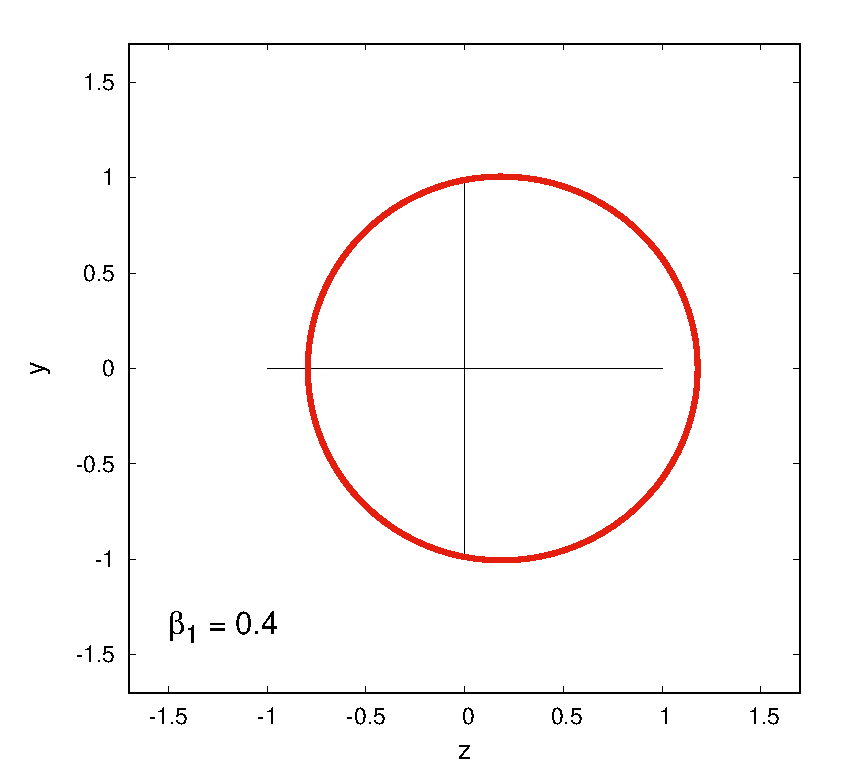
\includegraphics[width=6cm]{s1.eps}
    \hspace{1cm}
    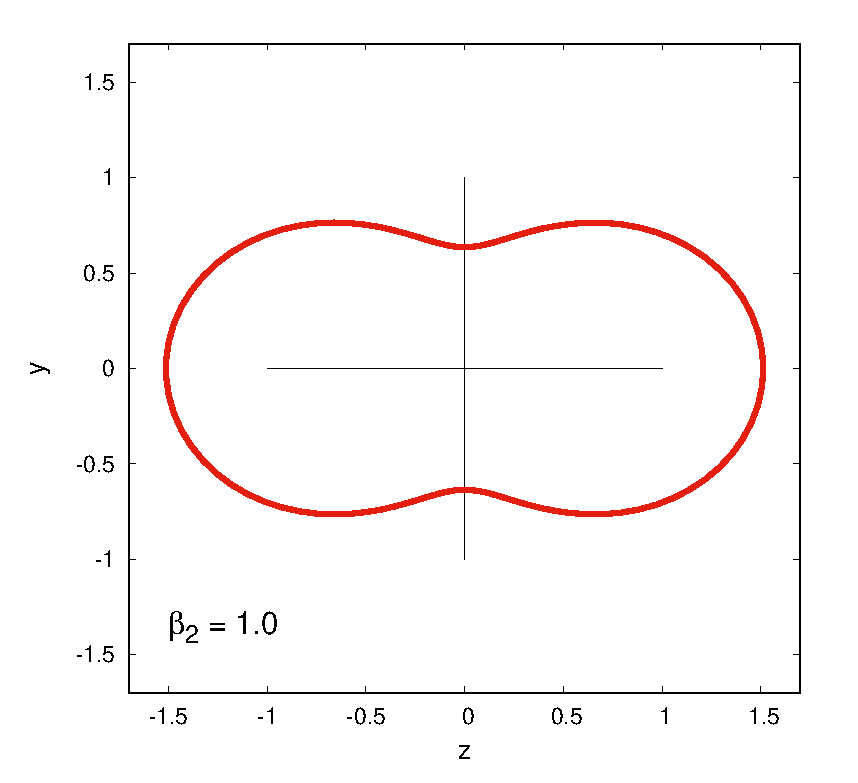
\includegraphics[width=6cm]{s2.eps}\\    
    \vspace{1.5cm}
    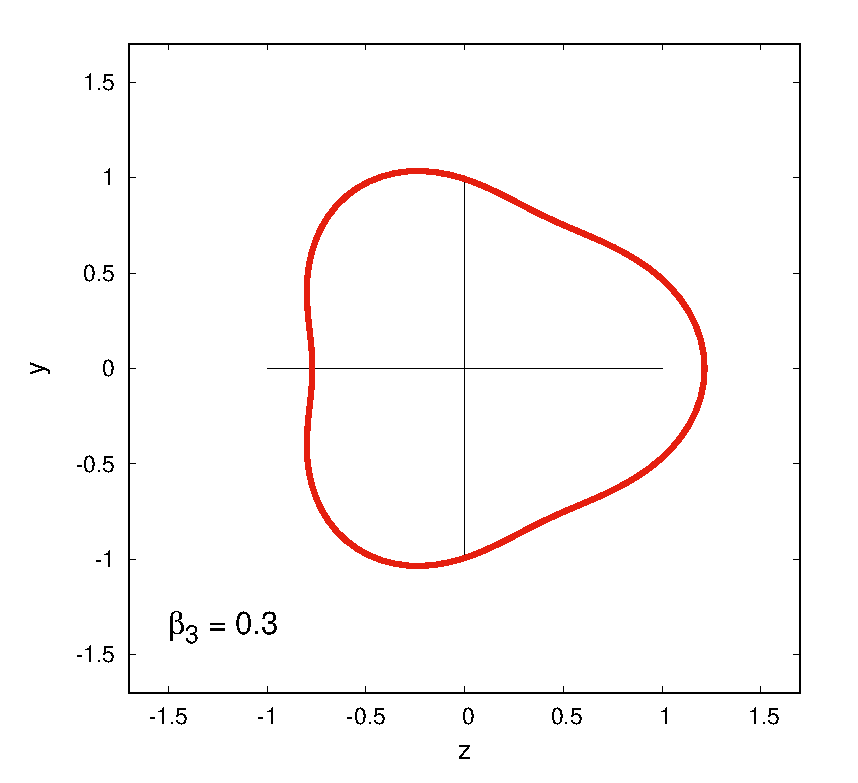
\includegraphics[width=6cm]{s3.eps}
    \hspace{1cm}
    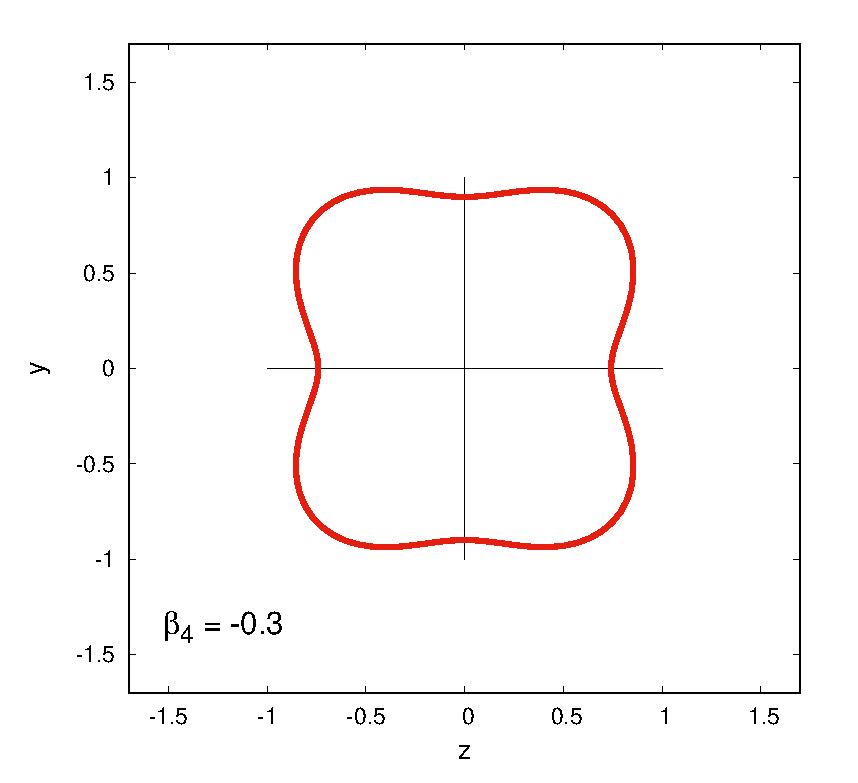
\includegraphics[width=6cm]{s4.eps}\\    
    \vspace{1.5cm}    
    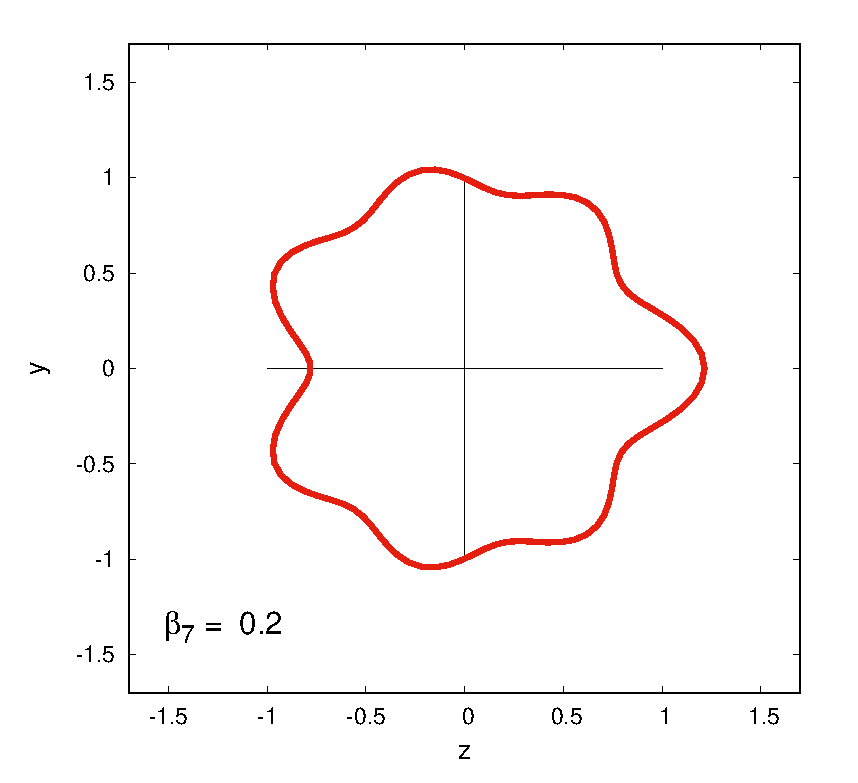
\includegraphics[width=6cm]{s5.eps}
    \hspace{1cm}
    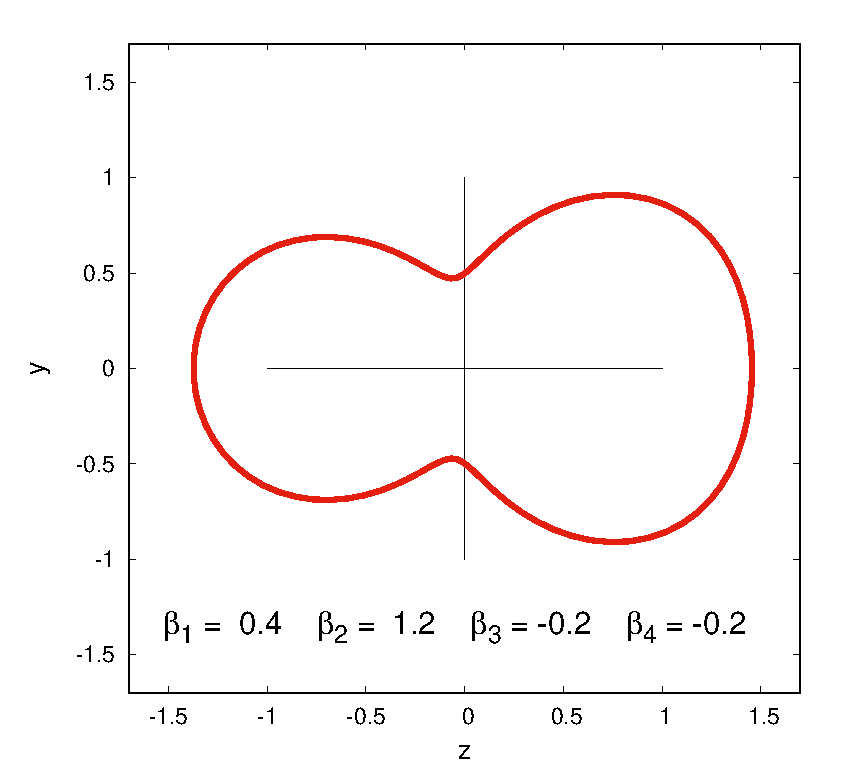
\includegraphics[width=6cm]{s6.eps}\\
    \vspace{1.5cm}    
    \caption{Przykładowe przekroje kształtów osiowosymetrycznych ($\mu=0$) względem płaszczyzny $\{y-z\}$, uzyskane w ramach parametryzacji $\beta$. W każdym 
    z przypadków użyte niezerowe parametry $\beta_{\lambda \mu}$ podawane są 
    w lewej dolnej części danego rysunku.}
    \label{example1}
\end{figure}
\vspace*{\fill}

\subsection{Parametryzacja modified Funny-Hills}

Jednym z możliwych sposobów zmniejszenia liczby parametrów w obliczeniach numerycznych energii jąder znajdujących się w stanach charakteryzujących się znacznym wydłużeniem może być użycie parametryzacji Funny-Hills \cite{OLDMFH}, lub jej zmodyfikowanej wersji, tj. modified Funny-Hills \cite{MFH}. W takim podejściu kształt rozszczepiającego się jądra definiowany jest za pomocą rozwinięcia w szereg wielomianów Lagrange'a~$P_{n}$:

\begin{equation} \label{eq:MFH1}
\tilde{\rho}^{2}_{s}(z)=R_{0}^{2}\sum_{n=0}^{\infty}\alpha_{n}P_{n}\left(\frac{z-z_{sh}}{z_{0}}\right),
\end{equation}
gdzie $\tilde{\rho}_{s}(z)$ jest odległością między osią symetrii jądra $z$ a jego powierzchnią. Początek i koniec tak zdefiniowanej bryły znajduje się odpowiednio w punktach: $z_{sh}-z_{0}$ oraz $z_{0}+z_{sh}$, co prowadzi do następujących zależności między współczynnikami rozwinięcia $\alpha_{n}$:
\begin{equation} \label{eq:MFH2}
\alpha_{0}=-\sum_{n=2,4,}^{\infty}\alpha_{n}, \qquad \alpha_{1}=-\sum_{n=3,5,}^{\infty}\alpha_{n}.
\end{equation}
Parametr $z_{sh}$ w (\ref{eq:MFH1}), odpowiadający za przesunięcie względem osi $z$, ustala środek masy jądra w punkcie $z=0$ i definiowany jest jako:

\begin{equation} \label{eq:MFH3}
z_{sh}=-\frac{1}{3}\frac{\alpha_{1}}{\alpha_{0}}z_{0}=-\frac{2}{9}\frac{\alpha_{1}}{\alpha_{0}^{2}}R_{0}.
\end{equation}
$R_{0}$, tak jak i w rozwinięciu (\ref{spherical}), jest promieniem jądra sferycznego. Warunek zachowania objętości bryły ulegającej deformacji prowadzi tu do zależności:
\begin{equation} \label{eq:MFH4}
z_{0}=\frac{2}{3}\frac{R_{0}}{\alpha_{0}},
\end{equation}
gdzie $z_{0}$ wyznacza połowę długości zdeformowanego jądra względem osi $z$. Dla $\lambda\leq4$ rozwinięcie (\ref{eq:MFH1}) odpowiada parametryzacji Funny-Hills \cite{OLDMFH}, gdzie dodatnie wartości parametru $B$ opisują formowanie się tzw. szyjki jądra podczas rozszczepienia: 

\begin{equation} \label{eq:MFH6}
\tilde{\rho}^{2}_{s}(z)=R_{0}^{2}c^{2}(1-u^{2})(A+\alpha u+Bu^{2}),
\end{equation}
przy założeniu, że $u=(z-z_{sh}) /z_{0}$.
Wartości ujemne $B$ odpowiadają natomiast kształtom przypominającym diament:
\begin{equation} \label{eq:MFH7}
\tilde{\rho}^{2}_{s}(z)=R_{0}^{2}c^{2}(1-u^{2})(A+\alpha u)e^{(Bc^{3}u^{2})}.
\end{equation}

Ze względu na fakt, że w niektórych przypadkach równania (\ref{eq:MFH6}) i (\ref{eq:MFH7}) prowadzić mogą do ujemnych (tj. niefizycznych) wartości $\tilde{\rho}^{2}_{s}(z)$, K. Pomorski i J. Bartel zaproponowali wprowadzenie poprawionej (zmodyfikowanej) wersji opisanej powyżej parametryzacji, tj. modified Funny-Hills:
\begin{equation} \label{eq:MFH8}
\tilde{\rho}^{2}_{s}(z)=\frac{R_{0}^{2}}{c f(a,B)}(1-u^{2})(1+\alpha u-Be^{-a^{2}u^{2}}),
\end{equation}
gdzie funkcja
\begin{equation} \label{eq:MFH9}
f(a,B)=1-\frac{3B}{4a^{2}}\left[e^{-a^{2}}+\sqrt{\pi}(a-\frac{1}{2a})Erf(a)\right],
\end{equation}
zapewnia normalizację objętości zdeformowanego nuklidu. Stała $z_{sh}$ wyznaczana jest wówczas z warunku zachowania objętości:

\begin{equation}
z_{sh}=- \frac{4}{15} \alpha ~ z_0 / f(a,B).
\end{equation}
Tak wprowadzona definicja (\ref{eq:MFH8}) jest teraz całkowicie wolna od ww. wad i pozwala na opis zarówno kształtów przypominających diament jak i tych charakteryzujących się przewężeniem (tj. szyjką). Znaczenie poszczególnych parametrów deformacji w (\ref{eq:MFH8}) jest tu bardzo podobne do tych w oryginalnej wersji Funny-Hills, tj. zmienna $c$ opisuje wydłużenie, $B$ formowanie się ,,szyjki'', natomiast $\alpha$ asymetrię masową, tj. kształty typu ,,gruszka''. Dodatkowo, ze względu na fakt, że wiele np. najcięższych jąder preferuje nieosiowe kształty w okolicach pierwszych barier, oraz że występowanie takich kształtów jest jeszcze bardziej prawdopodobne w przypadku stanów rotacyjnych, parametry $c,B,\lambda$ powinny być dodatkowo uzupełnione także o możliwość opisu asymetrii osiowej. Zgodnie z \cite{MFH} uzyskać to można wprowadzając do definicji $\tilde{\rho}^{2}_{s}(z)$ dodatkowy parametr $\eta$ i zapisując wzór na promień nuklidu jako:

\begin{equation}\label{eq:MFHOST}
{\rho}^{2}_{s}(z,\phi)=\tilde{\rho}^{2}_{s}(z) \frac {\sqrt{1-\eta^2}}{\sqrt{1+\eta \cos(2 \phi)}}.
\end{equation}
Warto zauważyć, że w tym przypadku parametr $\eta$ może być tu także stosunkowo łatwo uzależniony od $z$ co dałoby możliwość opisu wyjątkowo egzotycznych i skomplikowanych kształtów jądrowych.

W niniejszej pracy stałą $a$ występującą w (\ref{eq:MFH9}) przyjęto  zgodnie z \cite{POM2}, tj. jako: 

\begin{equation}
a=4,5-2c, 
\end{equation}
oraz w postaci liniowej kombinacji 
$B$ i $c$ wprowadzono następującą
definicję parametru $h$ \cite{DOBROW}
\begin{equation}
h=B/(3c-1),
\end{equation}
opisującego formowanie się szyjki. Ostatecznie więc przedstawiona parametryzacja zależna jest tylko od 4 zmiennych: $c, h, \alpha, \eta$, które opisują różne typy kształtów. Przykładowe kształty osiowo symetryczne, tj. $\eta = 0$, uzyskane w ramach parametryzacji modified Funny-Hills przedstawiono na rys.~\ref{fig:example2} w postaci ich przekroju względem płaszczyzny $\{y-z\}$.

\vspace*{\fill}
\begin{figure}[h!]
    \centering
    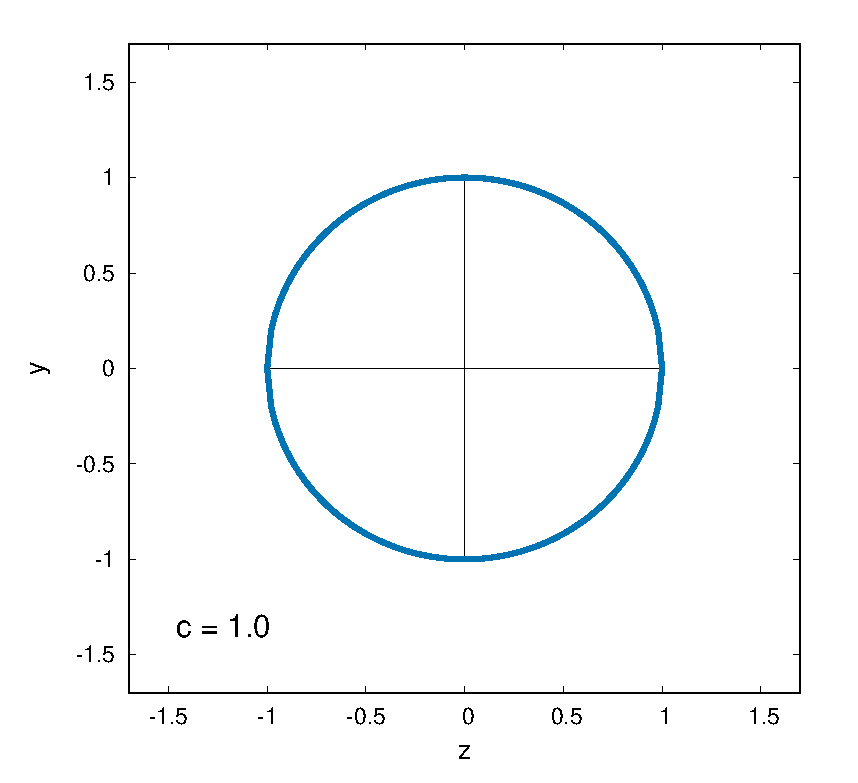
\includegraphics[width=6cm]{mfh1.eps}
    \hspace{1cm}
    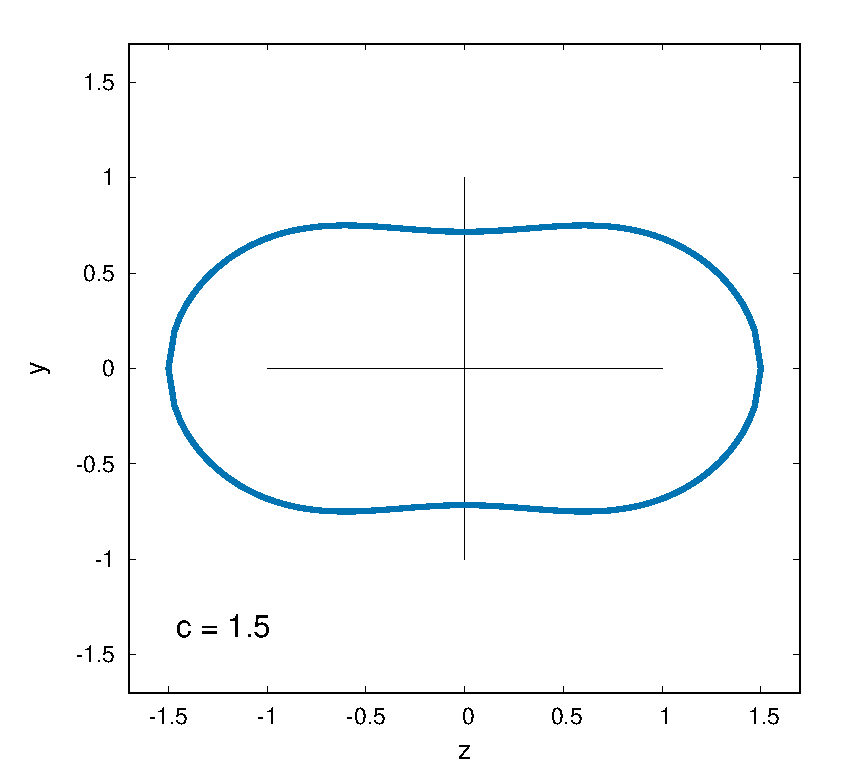
\includegraphics[width=6cm]{mfh2.eps}\\    
    \vspace{1.5cm}    
    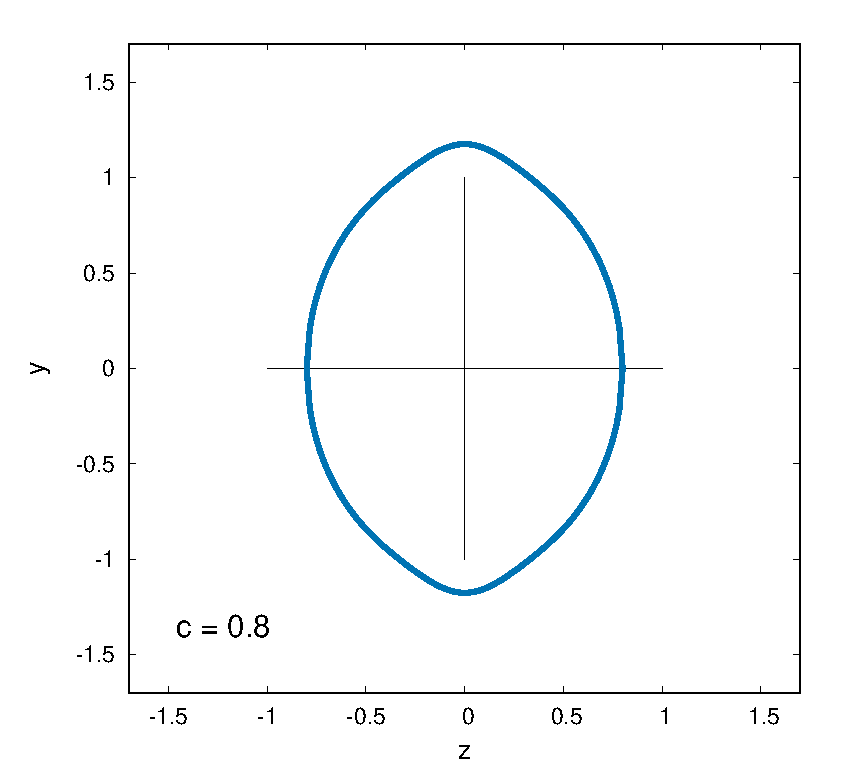
\includegraphics[width=6cm]{mfh3.eps}
    \hspace{1cm}
    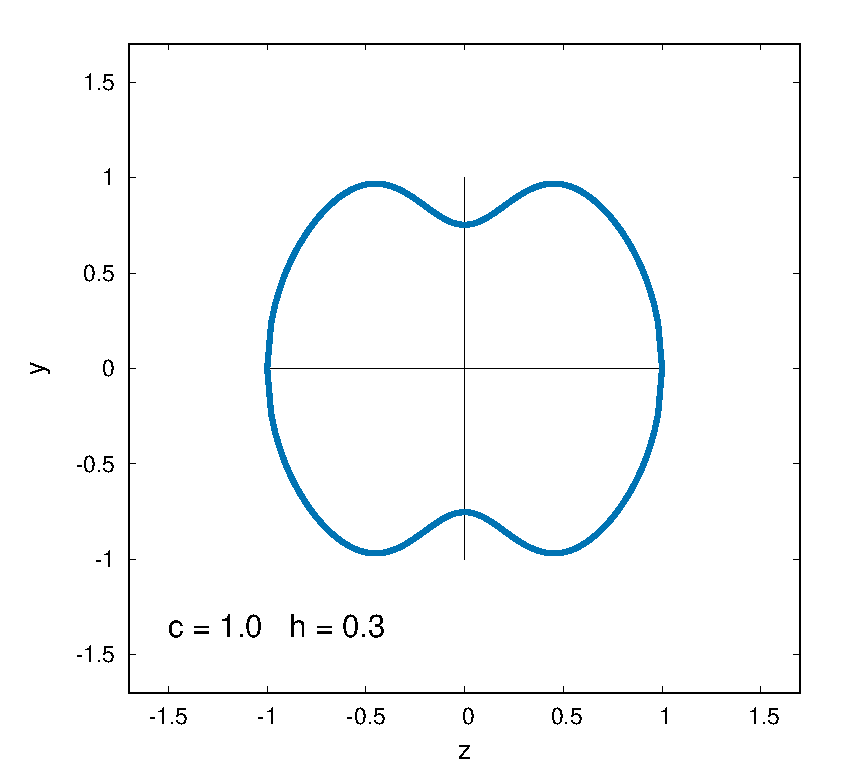
\includegraphics[width=6cm]{mfh4.eps}\\    
    \vspace{1.5cm}    
    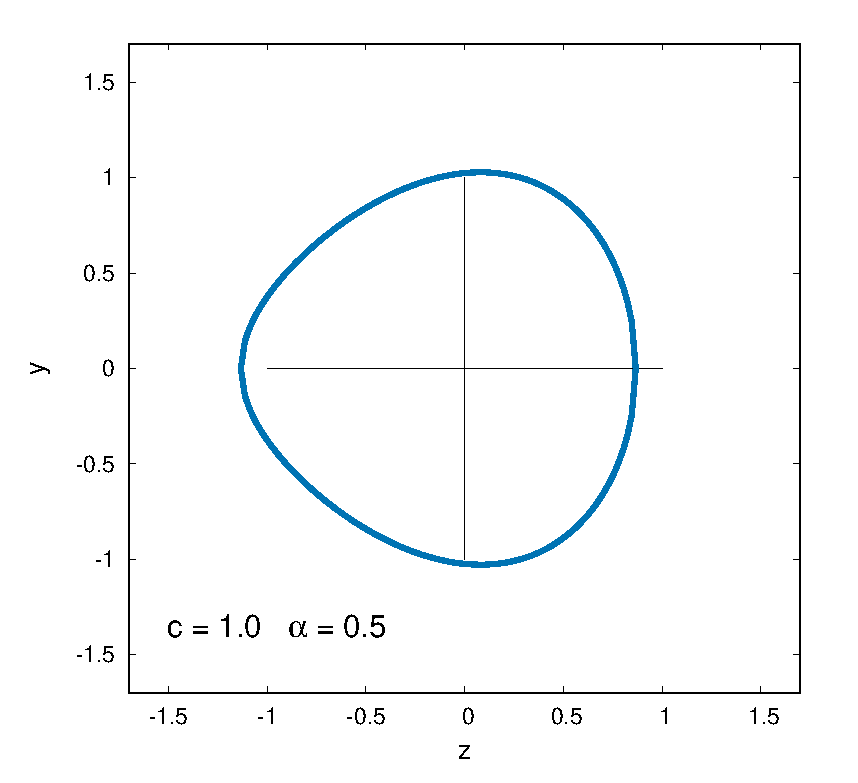
\includegraphics[width=6cm]{mfh5.eps}
    \hspace{1cm}
    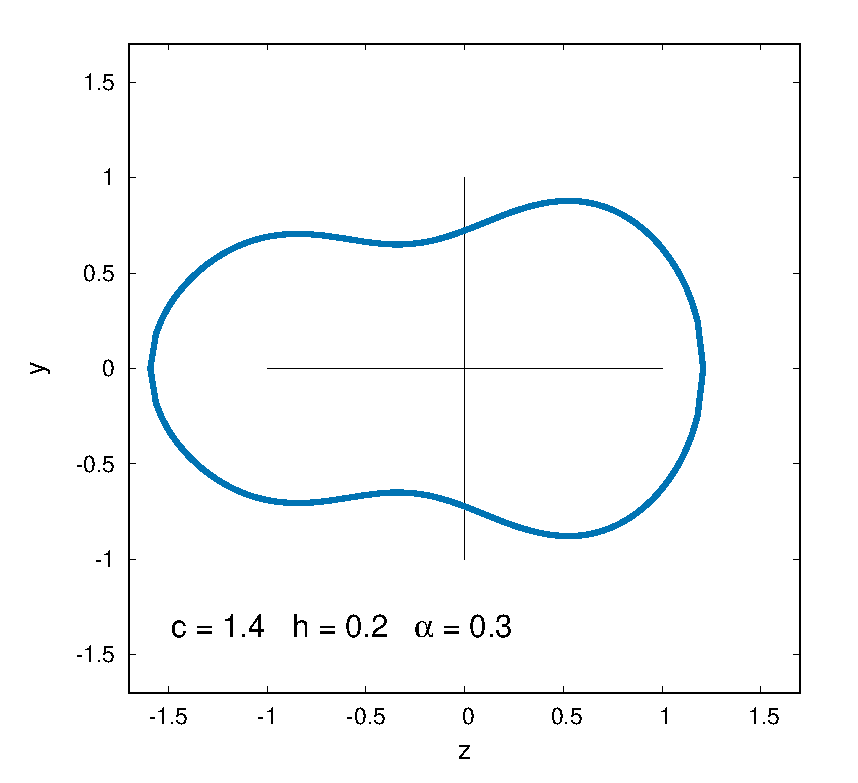
\includegraphics[width=6cm]{mfh6.eps}\\
    \vspace{1cm}
    \caption{Przykładowe przekroje kształtów osiowosymetrycznych ($\eta=0$ )względem płaszczyzny $\{y-z\}$, uzyskane w ramach parametryzacji modified Funny-Hills. W każdym 
    z przypadków użyte niezerowe parametry $c,h,\alpha$ podawane są w 
    lewej dolnej części danego rysunku.}
    \label{fig:example2}
\end{figure}
\vspace*{\fill}

\clearpage
\subsection{Konwersja kształtu modified Funny-Hills do rozwinięcia $\beta$}

Zgodnie z tym co zostało wcześniej powiedziane opisany przeze mnie w rozdziale 2 model makroskopowo-mikroskopowy, który będę wykorzystywał w niniejszej pracy, opiera się na parametryzacji $\beta$. Aby użyć go do wyznaczania energii/mas jąder w ramach parametryzacji modified Funny-Hills można np. zgodnie z \cite{Moll2009} wykorzystać fakt ortogonalności harmonik sferycznych $Y_{\lambda \mu}$, który pozwala na wyznaczenie parametrów $\beta_{\lambda \mu}$, dla dowolnego kształtu zadanego przez $r(\theta, \phi)$ w dowolnie przyjętej parametryzacji, w oparciu o wzór:

\begin{equation}
\beta_{\lambda \mu}=\sqrt{4\pi}\frac{\int r(\theta,\phi)Y_{\lambda \mu}
(\theta,\phi)\mathrm{d}\Omega}{\int r(\theta,\phi)Y_{0 0}(\theta,\phi)\mathrm{d}\Omega},
\end{equation}
którego dokładna postać używana w niniejszej pracy jest następująca:

\begin{equation}\label{przeliczanie}
\beta_{\lambda \mu}=\sqrt{4\pi}
\frac{\int_{0}^{2\pi}\int_{0}^{\pi}r(\theta,\phi)Y_{\lambda \mu}(\theta,\phi)\sin{\theta}\mathrm{d}\theta\mathrm{d}\phi}
{\int_{0}^{2\pi}\int_{0}^{\pi}r(\theta,\phi)Y_{0 0}(\theta,\phi)\sin{\theta}\mathrm{d}\theta\mathrm{d}\phi}.
\end{equation}
Całki widoczne w (\ref{przeliczanie}) rozwiązywał tu będę za pomocą 64-punktowej kwadratury Gaussa.

Otrzymane w ten sposób rozwinięcie powierzchni jądra w szereg harmonik sferycznych $Y_{\lambda \mu}$ jest oczywiście nieskończone. W praktyce oznacza to konieczność wybrania z (\ref{przeliczanie}) takiej liczby parametrów $\beta_{\lambda \mu}$ aby konwersja kształtu zadanego przez parametryzację modified Funny-Hills do parametryzacji $\beta$ była możliwie dokładna. Szczegółowe testy przeprowadzone w ramach niniejszej pracy wykazały, że na bardzo dokładną konwersję kształtów, zarówno bliskich sfery jak i charakteryzujących się znacznym wydłużeniem, pozwala w tym przypadku ograniczenie rozwinięcia (\ref{przeliczanie}) do następujących 27 parametrów $\beta_{\lambda \mu}$:

\begin{table}[h!]
\begin{center}
\begin{tabular}{ccccccccc}
%\hline
$\beta_{10}$ & $\beta_{20}$ & $\beta_{22}$ & $\beta_{30}$ & $\beta_{32}$ & $\beta_{40}$ & $\beta_{42}$ & $\beta_{44}$ & $\beta_{50}$\\
$\beta_{52}$ & $\beta_{54}$ & $\beta_{60}$ & $\beta_{62}$ & $\beta_{64}$ & $\beta_{66}$ & $\beta_{70}$ & $\beta_{72}$ & $\beta_{74}$\\
$\beta_{76}$ & $\beta_{80}$ & $\beta_{82}$ & $\beta_{84}$ & $\beta_{86}$ & $\beta_{88}$ & $\beta_{90}$ & $\beta_{10 \,\, 0}$ & $\beta_{11 \,\, 0}$ \\
%\hline
\end{tabular}
\end{center}
\end{table}
Przykładowe rezultaty takiej konwersji, zarówno dla kształtów osiowych jak i nieosiowosymetrycznych, przedstawiono na początku następnego rozdziału. Dodatkowo warto także wspomnieć, że analogiczne przeliczenie kształtu zadanego parametryzacją modified Funny-Hills (lub inną) na parametryzację $\beta$ można by uzyskać np. także metodą najmniejszych kwadratów, stawiając warunek minimalizacji funkcji $S$:

\begin{equation}
S=\sum \limits_{i} \Big( r(\theta_i, \phi_i) - \sum \limits_{\lambda, \mu} \beta_{\lambda \mu}^{'} Y_{\lambda \mu}(\theta_i, \phi_i) \Big )^2,
\end{equation}
gdzie $\beta_{\lambda \mu}^{'}$ oznaczają współczynniki $\beta_{\lambda \mu}$ przed normalizacją, tj. $\beta_{\lambda \mu}=\beta_{\lambda \mu}^{'}/\beta_{0 0}$. 

\clearpage
\section{Wyniki}

\subsection{Przykłady konwersji kształtu modified Funny-Hills do rozwinięcia \boldmath{$\beta$}}

Zasadniczym testem konwersji opartej na (\ref{przeliczanie}) może być porównanie kształtu zadanego przez parametryzację modified Funny-Hills z kształtem uzyskanym w parametryzacji $\beta$. W ramach niniejszej pracy przeprowadzono wiele tego typu testów, a poniżej na rys.~\ref{osiowy} przestawiony został rezultat jednego z nich, który na początek wykonałem w wersji osiowosymetrycznej. Przykładowy kształt w parametryzacji modified Funny-Hills jest w tym przypadku zdefiniowany przez:
\begin{gather*}
c=1,4, \qquad h=0,2, \qquad \alpha=0,3, \qquad \eta=0,0
\end{gather*}
i przedstawiony na rys.~\ref{osiowy} w postaci przekroju względem płaszczyzny $\{y-z\}$ za pomocą niebieskiej linii. Odpowiadający mu kształt w parametryzacji $\beta$, wyznaczony przy użyciu napisanego przeze mnie kodu numerycznego w języku Fortran, definiowany jest przez następujące wartości 27 parametrów $\beta_{\lambda \mu}$ uzyskanych z (\ref{przeliczanie}):

\begin{table}[h!]
\begin{center}
\begin{tabular}{llllll}
%\hline
$\beta_{10}= 0,080$ & $\beta_{20}= 0,769$  & $\beta_{22}= 0,000$  & $\beta_{30}=-0,336$ &  $\beta_{32}= 0,000$        & $\beta_{40}= 0,009$ \\
$\beta_{42}= 0,000$ & $\beta_{44}= 0,000$  & $\beta_{50}=-0,016$ & $\beta_{52}=  0,000$  & $\beta_{54}= 0,000$        & $\beta_{60}=-0,018$ \\     
$\beta_{62}= 0,000$ & $\beta_{64}= 0,000$  & $\beta_{66}= 0,000$  & $\beta_{70}= 0,038$  & $\beta_{72}= 0,000$        & $\beta_{74}= 0,000$  \\ 
$\beta_{76}= 0,000$ & $\beta_{80}=-0,006$ & $\beta_{82}=  0,000$  & $\beta_{84}= 0,000$  & $\beta_{86}= 0,000$        & $\beta_{88}= 0,000$ \\ 
$\beta_{90}=-0,008$& $\beta_{10 \,\, 0}= 0,007$ & $\beta_{11 \,\, 0}=-0,008$ &   &   &                    \\
%\hline
\end{tabular}
\end{center}
\end{table}
\noindent
i zaznaczony na rys.~\ref{osiowy} za pomocą czerwonych kropek. Widać, że konwersja oparta na metodzie (\ref{przeliczanie}) działa w tym przypadku właściwie, gdyż oba przekroje widoczne na rys.~\ref{osiowy} pokrywają się z dużą dokładnością. Dodatkowo można także zauważyć, że zgodnie z oczekiwaniem, wszystkie wyznaczone tu $\beta_{\lambda \mu}$ z  $\mu \neq 0$ są równe $0$ ze względu na przyjęcie $\eta=0$.

\begin{figure}[ht!]
\centering
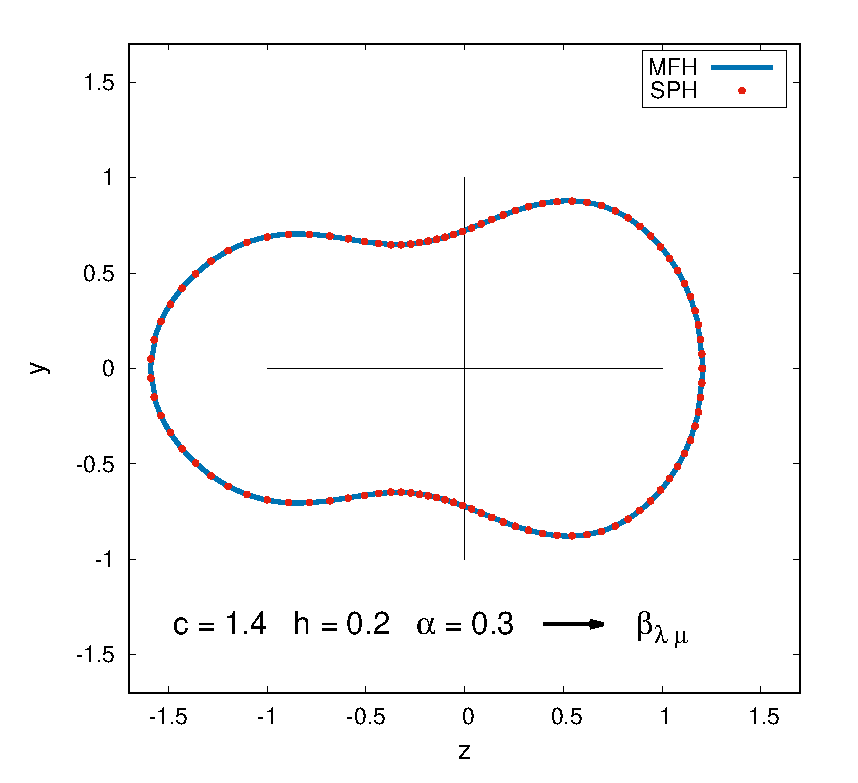
\includegraphics[height=10cm]{axial.eps}
\caption{Przykład konwersji kształtu osiowosymetrycznego w przekroju $\{y-z\}$ z parametryzacji modified Funny-Hills (MFH), oznaczonego niebieską linią, do kształtu w parametryzacji $\beta$ (SPH), oznaczonego czerwonymi kropkami.}
\label{osiowy}
\end{figure}
\bigskip
\noindent
Analogiczną konwersję wykonać można także oczywiście i dla kształtów łamiących symetrię osiową. Na rys.~\ref{fig:example3} przedstawiony został właśnie tego typu przypadek, tj. kształt w parametryzacji modified Funny-Hills jest tam definiowany przez:
\begin{equation}
c=1,4, ~~~h=0,2, ~~~\alpha=0,2, ~~~\eta=-0,3 \nonumber
\end{equation}
i zaznaczony kolorem niebieskim, natomiast kształt otrzymany w parametryzacji $\beta$ oznaczony jest kolorem czerwonym i odpowiadają mu następujace wartości wyznaczonych $\beta_{\lambda \mu}$:
\begin{table}[h!]
\begin{center}
\begin{tabular}{llllll}
%\hline
$\beta_{10}= 0,062$ & $\beta_{20}= 0,845$  & $\beta_{22}= 0,305$  & $\beta_{30}=-0,238$ &  $\beta_{32}= 0,000$        & $\beta_{40}=-0,029$ \\
$\beta_{42}= 0,114$ & $\beta_{44}= 0,031$  & $\beta_{50}=-0,005$ & $\beta_{52}= -0,042$  & $\beta_{54}= 0,000$        & $\beta_{60}=-0,027$ \\     
$\beta_{62}=-0,008$ & $\beta_{64}= 0,013$  & $\beta_{66}= 0,004$  & $\beta_{70}= 0,028$  & $\beta_{72}= 0,002$        & $\beta_{74}=-0,006$  \\ 
$\beta_{76}= 0,000$ & $\beta_{80}= 0,007$ & $\beta_{82}= -0,008$  & $\beta_{84}=-0,001$  & $\beta_{86}= 0,002$        & $\beta_{88}= 0,000$ \\ 
$\beta_{90}=-0,010$& $\beta_{10 \,\, 0}= 0,005$ & $\beta_{11 \,\, 0}=-0,004$ &   &   &                    \\
%\hline
\end{tabular}
\end{center}
\end{table}

wśród których wiele $\beta_{\lambda \mu}$ charakteryzujących się $\mu \neq 0$ ma niezerową wartość, ze względu na przyjęcie $\eta=-0,3$. Także i w tym przypadku oba kształty widoczne na rys.~\ref{fig:example3}, przedstawione w czterech kolejnych rzutach, pokrywają się z dużą dokładnością, co stanowi potwierdzenie poprawności działania napisanego przeze mnie kodu opartego na konwersji zgodnej z (\ref{przeliczanie}). Dodatkowo w celu lepszego zobrazowania pokrywania się kształtów z rys.~\ref{fig:example3}, na rys.~\ref{przekroje} pokazane zostały ich przekroje względem płaszczyzn: $\{x-y\}$ oraz $\{y-z\}$.


\vspace*{\fill}
\begin{figure}[ht!]
    \centering
    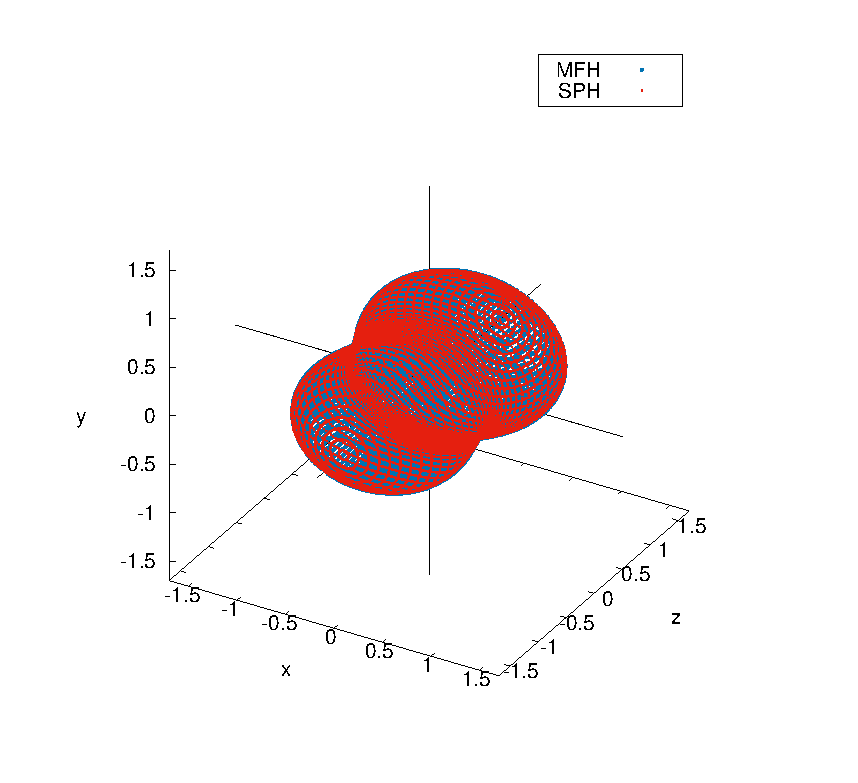
\includegraphics[width=7cm]{rys1.eps}    
    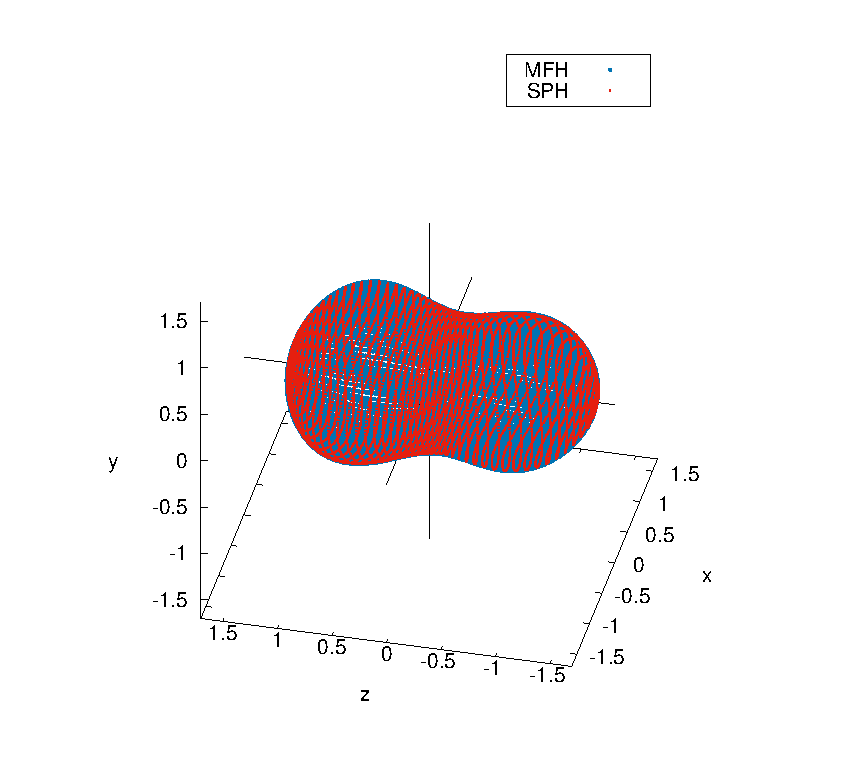
\includegraphics[width=7cm]{rys2.eps}\\    
    \vspace{1.5cm}    
    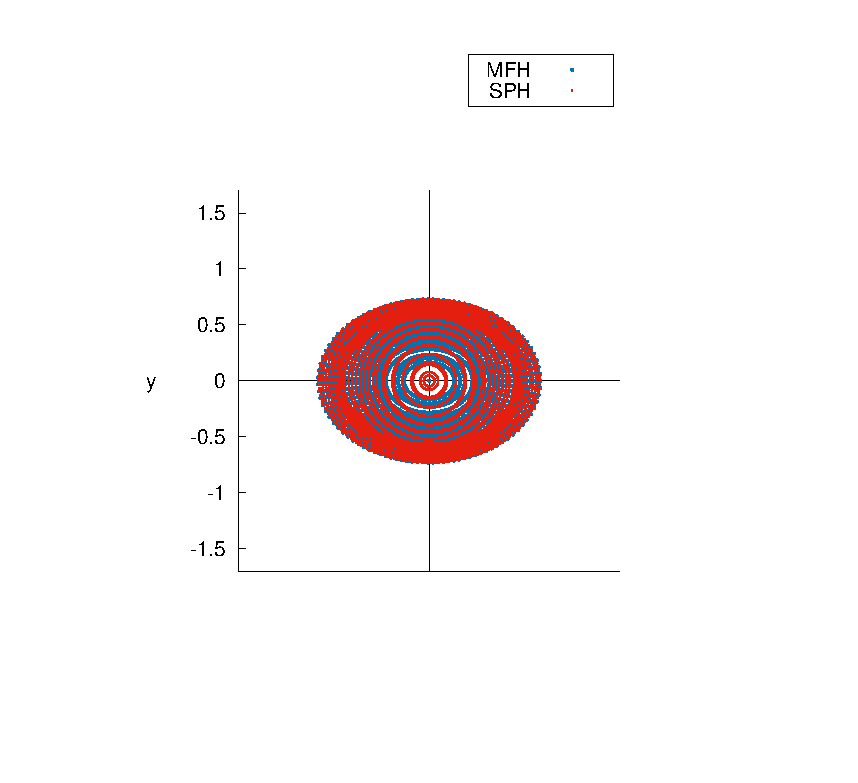
\includegraphics[width=7cm]{rys3.eps}
    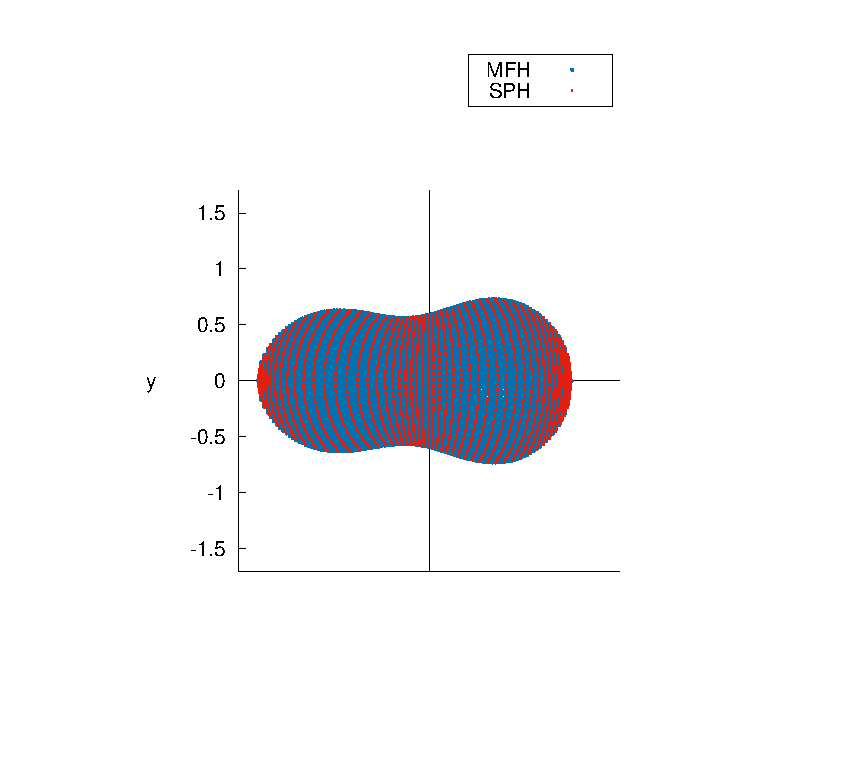
\includegraphics[width=7cm]{rys4.eps}\\
    \vspace{0.5cm}    
	\caption{Przykład konwersji kształtu łamiącego symetrię osiową, zadanego parametryzacją modified Funny-Hills (MFH) i oznaczonego niebieskimi kropkami, do kształtu w parametryzacji $\beta$ (SPH), oznaczonego czerwonymi kropkami.}
    \label{fig:example3}%
\end{figure}
\vspace*{\fill}




\vspace*{\fill}
\begin{figure}[ht!]
    \centering
    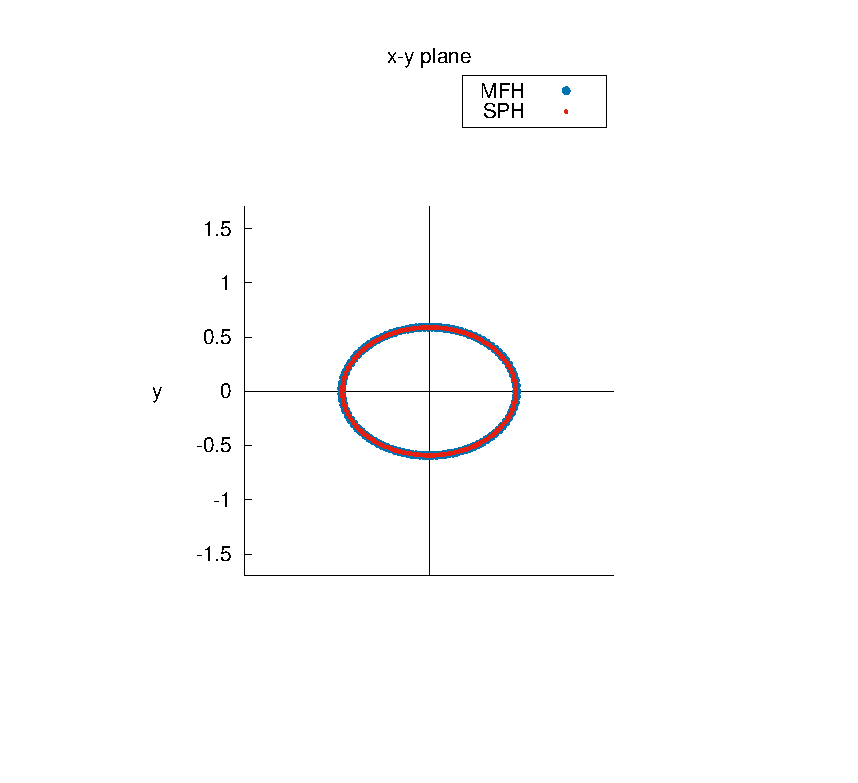
\includegraphics[width=7.2cm]{xy_plane.eps}    
    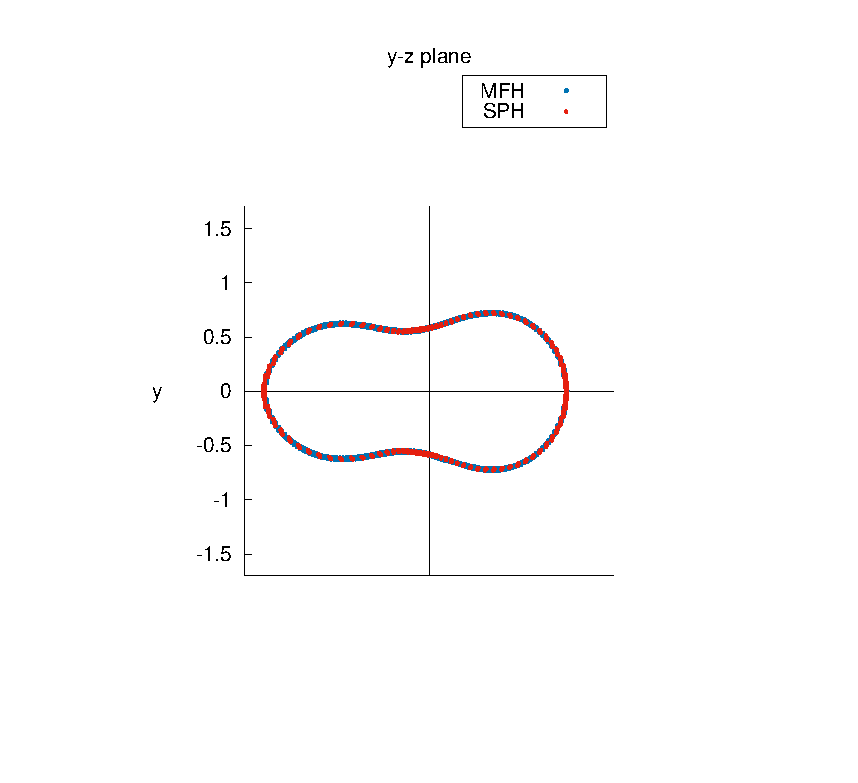
\includegraphics[width=7.2cm]{yz_plane.eps}\\    
	\caption{Przekroje kształtów z rys.~\ref{fig:example3} względem płaszczyzn: $\{x-y\}$ oraz $\{y-z\}$. Kropki niebieskie oznaczają kształt zadany parametryzacją modified Funny-Hills (MFH), natomiast kształt w parametryzacji $\beta$ (SPH) oznaczony jest kropkami czerwonymi}
    \label{przekroje}%
\end{figure}
\vspace*{\fill}



\subsection{Obliczenia mas dla stanów podstawowych}

Opisana powyżej umiejętność dokładnego przeliczania kształtu zdefiniowanego w parametryzacji modified Funny-Hills na parametryzację $\beta$, umożliwiła mi wyznaczanie energii/masy danego jądra dla dowolnie przyjętych parametrów $c, h, \alpha, \eta$, wykorzystując opisany w rozdziale 2 model makroskopowo-mikroskopowy, którego numeryczna implementacja opiera się właśnie na parametryzacji $\beta$. Ponieważ celem mojej pracy było zbadanie czy parametryzacja modified Funny-Hills dobrze sprawdzi się przy wyznaczaniu mas/energii stanów podstawowych, jako kandydatów do testów wybrałem trzy jądra, z których dwa tj. $^{238}U$, $^{222}Rn$ są stosunkowo dobrze znane eksperymentalnie, natomiast trzecie $^{173}123$ nie zostało jak dotąd zaobserwowane. Jądro $^{238}U$ wybrałem ze względu na oczekiwany, np. zgodnie z \cite{RIPL3}, niewielki stopień komplikacji jego kształtu w stanie podstawowym, tj. nieduża deformacja kwadrupolowa z domieszką deformacji hexadekapolowej. Jądro $^{222}Rn$ oprócz wymienionych dla $^{238}U$ dwóch głównych typów deformacji powinno dodatkowo charakteryzować się w stanie podstawowym niezerową deformacją oktupolową, ze względu na rezultaty licznych eksperymentów takich jak np. \cite{E3}. Ostatnie hipotetyczne jądro $^{173}123$, zgodnie z przewidywaniami \cite{A32}, powinno charakteryzować się w stanie podstawowym bardzo egzotycznym kształtem, przypominającym spłaszczony sferoid o lekko trójkątnym równiku. 

Aby w ramach parametryzacji modified Funny-Hills wyznaczyć energie/masy w stanach podstawowych wymienionych jąder, oraz deformacje takich punktów, należy znaleźć minimum energii danego jądra, leżące przed odpowiadającą mu barierą rozszczepieniową, względem parametrów $c, h,\alpha, \eta$. Wykorzystać w tym celu można dowolną procedurę minimalizacyjną, lub posłużyć się siecią energii potencjalnej (w tym przypadku 4-wymiarową, zależną od $c, h,\alpha, \eta$) i znaleźć na niej odpowiednie minimum. W niniejszej pracy wykorzystałem drugą z wymienionych metod i dla każdego z trzech wybranych do testu jąder wygenerowałem sieć energii potencjalnej o następujących zakresach w poszczególnych parametrach deformacji:
\begin{align*}
c&=0,70~(0,05)~1,40,\\
h&=-0,25~(0,05)~0,25,\\
\alpha&=0,00~(0,05)~0,95,\\
\eta&=0,00~(0,05)~0,30,
\end{align*}
gdzie wartości w nawiasach oznaczają przyjęty krok dla każdej ze zmiennych. Widać więc, że przyjęty tu krok był zawsze równy 0,05. Wyznaczoną energię na tak zdefiniowanej sieci wyrysowywałem następnie dla każdego z badanych jąder w trzech kolejnych rzutach, tj. $\{c,h\}$, $\{c, \alpha\}$ oraz $\{c, \eta\}$, z których w kroku następnym, ręcznie odczytywałem energię/masę w stanie podstawowym oraz odpowiadające takiemu punktowi parametry deformacji.

\clearpage
\subsubsection{\textsuperscript{238}U}

Postępując w sposób opisany powyżej i bazując na analizie rzutów energii potencjalnej widocznych na rys.~\ref{uran} w przypadku jądra $^{238}U$ otrzymałem następujące wartości parametrów deformacji dla jego stanu podstawowego:
\begin{equation*}
c=1,20, \quad h=-0,10, \quad \alpha=0,00, \quad \eta= 0,00
\end{equation*}
przy odpowiadającej mu masie równej $M=47,585$ MeV. Zgodnie z danymi eksperymentalnymi, np. \cite{brookhaven}, zmierzona masa tego jądra w stanie podstawowym jest równa $47,308$ MeV. Otrzymany przeze mnie wynik jest więc nieznacznie zawyżony względem wartości eksperymentalnej i różni się od niej o $277$ keV. Warto także zauważyć, że do tak dokładnego wyznaczenia masy w stanie podstawowym tego jądra wystarczyły tu tylko dwie zmienne w parametryzacji modified Funny-Hils, tj. $c$ oraz $h$, podczas gdy np. w standardowym rozwinięciu w harmoniki sferyczne wymagane byłoby tu użycie co najmniej 4 parametrów $\beta_{\lambda \mu}$, tj. $\beta_{20},\beta_{40},\beta_{60},\beta_{80}$, np. \cite{JACHBF}.


\begin{figure}[h!]
\centering
\includegraphics[height=6.5cm]{238U_c_h.eps}
\includegraphics[height=6.5cm]{238U_c_alpha.eps}
\includegraphics[height=6.5cm]{238U_c_eta.eps}
\caption{Powierzchnia energii potencjalnej dla $^{238}U$, zależna od $c,h,\alpha,\eta$, w trzech kolejnych rzutach, tj. $\{c,h\}$, $\{c,\alpha\}$ oraz $\{c,\eta\}$. }
\label{uran}
\end{figure}


\subsubsection{\textsuperscript{222}Rn}

Bazując na analogicznych rzutach energii potencjalnej dla jądra $^{222}Rn$, przedstawionych na rys.~\ref{radon}, otrzymałem następujące wartości parametrów deformacji dla jego stanu podstawowego:
\begin{equation*}
c=1,15, \quad h=-0,05, \quad \alpha=0,60, \quad \eta= 0,00,
\end{equation*}
oraz odpowiadającą mu masę równą $M=16,769$ MeV. Tak jak i w przypadku $^{238}U$, otrzymany przeze mnie rezultat jest tu nieznacznie zawyżony w stosunku do wartości eksperymentalnej, wynoszącej $16,372$ MeV \cite{brookhaven}. Wynikająca stąd różnica jest zatem równa $397$ keV. Dodatkowo warto także zauważyć, że zgodnie z opisanymi wcześniej przewidywaniami, kształt tego jądra w stanie podstawowym charakteryzuje się większym stopniem komplikacji niż miało to miejsce w przypadku $^{238}U$, tj. do jego opisu wymagane są tu trzy parametry: $c$, $h$, oraz dodatkowo $\alpha$. 


\begin{figure}[h!]
\centering
\includegraphics[height=6.5cm]{222Rn_c_h.eps}
\includegraphics[height=6.5cm]{222Rn_c_alpha.eps}
\includegraphics[height=6.5cm]{222Rn_c_eta.eps}
\caption{Powierzchnia energii potencjalnej dla $^{222}Rn$, zależna od $c,h,\alpha,\eta$, w trzech kolejnych rzutach, tj. $\{c,h\}$, $\{c,\alpha\}$ oraz $\{c,\eta\}$. }
\label{radon}
\end{figure}


\subsubsection{\textsuperscript{296}123}

Ostatnim ze zbadanych przeze mnie jąder był hipotetyczny układ $^{296}123$, którego trzy kolejne rzuty energii potencjalnej przedstawione zostały na rys.~\ref{123}. Mapy te różnią się od tych dla: $^{238}U$ oraz $^{222}Rn$ faktem występowania na nich dwóch porównywalnych (w sensie energii) minimów, z których jedno charakteryzuje się lekką deformacją typu oblate ($c=0,90$), natomiast drugie egzotycznym kształtem wyznaczanym przez niezerowe wartości parametrów $c, \alpha$ i $\eta$. Niewiele niższe jest tu to drugie (egzotyczne) minimum a odczytane z rys.~\ref{123} odpowiadające mu parametry deformacji są następujące:
\begin{equation*}
c=1,05, \quad h= 0,00, \quad \alpha=0,10, \quad \eta= 0,15,
\end{equation*}
oraz uzyskana przeze mnie  masa w tym punkcie równa $237,363$ MeV. Masy tej (z oczywistych względów) nie da się porównać z wynikiem uzyskanym na drodze eksperymentu, jednakże rezultaty zawarte w pracy \cite{A32} wskazują, że uzyskany tu kształt oraz masa w stanie podstawowym wydają się być właściwe. Zgodnie z \cite{A32} kształt ten powinien charakteryzować się niezerową wartością parametrów $c, \alpha$ i $\eta$, przy odpowiadającej im masie w stanie podstawowym równej $237,007$ MeV. Dane te są więc w dużej zgodzie z rezultatem otrzymanym przeze mnie. 

\begin{figure}[h!]
\centering
\includegraphics[height=6.5cm]{296_123_c_h.eps}
\includegraphics[height=6.5cm]{296_123_c_alpha.eps}
\includegraphics[height=6.5cm]{296_123_c_eta.eps}
\caption{Powierzchnia energii potencjalnej dla hipotetycznego jądra $^{296}123$, zależna od $c,h,\alpha,\eta$, w trzech kolejnych rzutach, tj. $\{c,h\}$, $\{c,\alpha\}$ oraz $\{c,\eta\}$. }
\label{123}
\end{figure}

\clearpage
\section{Wnioski}

W chwili obecnej najlepsze globalne oszacowania teoretyczne mas znanych jąder dostarczają rezultatów charakteryzujących się $\delta_{rms}$ rzędu 500-800 keV względem danych empirycznych. Wartość ta w przypadku podejścia Hartree-Fock-Bogoliubov \cite{Gor1,Gor2} jest równa $\delta_{rms}$ = 0,729 MeV, obliczenia makroskopowo-mikroskopowe w obszarze od O do Hs wykonywane przez P. M\"oller'a i innych \cite{Moll2009} dają  $\delta_{rms}$=0,669 MeV, natomiast fenomenologiczna formuła autorstwa Duflo i Zuker'a \cite{Duflo} prowadzi do $\delta_{rms}$=0,574 MeV. Oczywiście istnieją sposoby na zmniejszenie wartości wymienionych tu błędów rms, jednakże najczęściej wiąże się to z wprowadzeniem do danego modelu kilku kolejnych poprawek, które bardzo łatwo mogą zaburzyć jego sens fizyczny. W tym kontekście uzyskane przeze mnie rezultaty dotyczące mas w stanach podstawowych jąder $^{222}Rn$ oraz $^{238}U$ mimo, że różnią sie od wartości eksperymentalnych o odpowiednio: $397$ keV oraz $277$ keV, stanowią więc bardzo dobry wynik i potwierdzenie, że użyta tu parametryzacja modified Funny-Hills jest skutecznym sposobem na proste, a zarazem dokładne, wyznaczenie masy/energii stanu podstawowego przy użyciu niewielkiej liczby parametrów opisujących kształt danego nuklidu. Warto także zauważyć, że uzyskane tu rezultaty dla hipotetycznego jądra  $^{296}123$ w oparciu o wykorzystanie tylko 4 parametrów: $c, h, \alpha, \eta$, są bardzo zbliżone do tych uzyskanych w ramach parametryzacji $\beta$ \cite{A32}, bez opisanej tam konieczności posługiwania się aż 10 parametrami $\beta_{\lambda \mu}$. Oznacza to, że parametryzacja modified Funny-Hills sprawdza się nie tylko przy opisie typowych kształtów jakie występują w okolicach stanów podstawowych, lecz z powodzeniem opisywać może nawet te najbardziej egzotyczne, będące przejawem kwantowej natury układu nukleonów jakim jest jądro atomowe.

Kolejnym wnioskiem jaki można zauważyć analizując uzyskane przeze mnie wyniki jest fakt systematycznego zawyżania wartości mas w stanach podstawowych w ramach używanej tu parametryzacji modified Funny-Hills, względem: danych eksperymentalnych w przypadku $^{222}Rn$ i $^{238}U$, oraz w przypadku $^{296}123$ względem przewidywań z użyciem parametryzacji $\beta$. Efekt ten wynika przede wszystkim z niedokładności przyjętej tu procedury wyznaczania stanów podstawowych w oparciu o sieć o kroku 0,05 w każdym wymiarze. Zwiększając gęstość takiej sieci, tj. zmniejszając przyjęty przeze mnie krok, wyznaczone tu masy uległy by dodatkowemu obniżeniu, co prowadziłoby do ich jeszcze większej zgodności z \cite{A32} oraz \cite{brookhaven}.

Badana przeze mnie w niniejszej pracy parametryzacja modified Funny-Hills jest więc bardzo dobrym sposobem opisu okolic stanów podstawowych zarówno silnie jak i słabo zdeformowanych nuklidów. Jeszcze większą przydatność wykazywać będzie zapewne w przypadku znacznych wydłużeń, tj. kształtów bliskich rozszczepienia, czyli w obszarze jądrowych deformacji do których opisu parametryzacja ta została specjalnie przygotowana.

\clearpage
\begin{thebibliography}{9}

\bibitem{1935}
H. Sch{\"o}ler und Th. Schmidt, \textit{Z. Phys.}, \textbf{94}, 457 (1935);  \textbf{95}, 265 (1935).
\bibitem{1939}
N. Bohr, J. Wheeler, \textit{Phys. Rev.}, \textbf{56} (1939) 426.
\bibitem{parametryzacje}
R. W. Hasse, W. D. Myers, \textit{Geometrical Relationships of Macroscopic Nuclear Physics}, Springer-Verlag, Berlin, 1988. 
\bibitem{Jach1}
P. Jachimowicz, M. Kowal, and J. Skalski, \textit{Phys. Rev. C} \textbf{87}, 044308 (2013).
\bibitem{MFH}
K. Pomorski and J. Bartel, \textit{IJMPE} Vol. \textbf{15} No. 2, 417 (2006).
\bibitem{OLDMFH}
M. Brack, J. Damgaard, A. S. Jensen, H. C. Pauli, V. M. Strutinsky, C. Y. Wong, \textit{Rev. Mod. Phys.} \textbf{44}, 320 (1972).
\bibitem{NIX}
J. R. Nix, \textit{Nucl. Phys. A} \textbf{130}, 241 (1969).
\bibitem{Moll2009}
P. M{\"o}ller, A. J. Sierk, T. Ichikawa, A. Iwamoto, R. Bengtsson, H. Uhrenholt, and S. Aberg, \textit {Phys. Rev. C} \textbf{79}, 064304 (2009).
\bibitem{JACHQ}
P. Jachimowicz, M. Kowal, and J. Skalski, \textit{Phys. Rev. C} \textbf{89}, 024304 (2014).
\bibitem{JACHBF}
P. Jachimowicz, M. Kowal, and J. Skalski, \textit{Phys. Rev. C} \textbf{95}, 014303 (2017).
\bibitem{Muntian}
I. Muntian, Z. Patyk, A. Sobiczewski, \textit{Acta Phys. Pol. B} \textbf{32}, 691 (2001).
\bibitem{Krappe}
H. J. Krappe, J. R. Nix, A. J. Sierk, \textit{Phys. Rev. C} \textbf{20}, 922 (1979).
\bibitem{Moll1}
P. M{\"o}ller, J. R. Nix, \textit{Nucl. Phys. A} \textbf{361}, 117 (1981).
\bibitem{Moll2}
P. M{\"o}ller, J. R. Nix, W. D. Myers, W. J. Świątecki, \textit{At. Data and Nucl. Data Tables} \textbf{59}, 185 (1995).
\bibitem{WS}
S. Ćwiok, J. Dudek, W. Nazarewicz, J. Skalski, T. Werner \textit{Comput. Phys. Commun.} \textbf{46}, 379 (1987).
\bibitem{Strutin}
V. M. Strutinsky, \textit{Sov. J. Nucl. Phys.} \textbf{3}, 449 (1966).
\bibitem{Pomorski}
Bożena Nerlo-Pomorska, Krzysztof Pomorski, \textit{Zarys teorii jądra atomowego}, PWN, Warszawa, 1999.
\bibitem{BCS}
A. Bohr, B. Mottelson, D. Pines, \textit{Phys. Rev. C} \textbf{110}, 936 (1958).
\bibitem{G}
S. G. Nilsson et. al, \textit{Nuc. Phys. A} \textbf{131}, 1 (1969).
\bibitem{POM2}
J. Bartel, K. Pomorski, \textit{Int. Journ. Mod. Phys. E} \textbf{17}, 100 (2008).
\bibitem{DOBROW}
A. Dobrowolski, K. Pomorski, J. Bartel, \textit{Physica Scripta T} \textbf{125}, 188 (2006). 
\bibitem{RIPL3}
https://www-nds.iaea.org/RIPL-3/
\bibitem{E3}
L. P. Gaffney et. al, \textit{Nature}  \textbf{497}, 199 (2013). 
\bibitem{A32}
P. Jachimowicz, M. Kowal, and J. Skalski, \textit{Phys. Rev. C} \textbf{95}, 034329 (2017).
\bibitem{brookhaven}
http://www.nndc.bnl.gov/
\bibitem{Gor1}       
S. Goriely, M. Samyn, and J.M. Pearson,  \textit{Phys. Rev. C} \textbf{75}, 064312 (2007).
\bibitem{Gor2}       
G. Audi, A.H. Wapstra, and C. Thibault,  \textit{Nucl. Phys. A} \textbf{729}, 337 (2003).
\bibitem{Duflo}     
J. Duflo and A.P. Zuker, \textit{Phys. Rev. C} \textbf{52}, 23 (1995).

\end{thebibliography}

\end{document}
